\tikzset{%
	every state/.style={
		draw=maincolor,
		thick,
		fill=maincolor!18,
		inner sep=.8ex,
		minimum size=0pt
	},	
	field/.style={
		state,
		shape aspect=5,
		shape=rectangle
	},
	success/.style={
		state,
		field,
		fill=green!60!black!50
	},
	error/.style={
		state,
		field,
		fill=purple!50
	},
	shorten >=1pt,
	initial text={}
}

\chapter{Testing}
\label{chap_testing}

\mode
<all>

\targets{
	\item Understand the basic principles of testing.
	\item Know how and when to use testing in software development.
	\item Understand code inspection and walkthroughs as human unit testing techniques.
}



\section{Principles of Testing}

\subsection*{Motivating Example}

\subsubsection*{Problem Definition}

\begin{Frame}{A little exercise (Myers)}
  \begin{itemize}
    \item Input: three integer values\\
      representing lengths of the sides of a triangle.
    \item Output: \texttt{scalene}, \texttt{isosceles}, or \texttt{equilateral}
  \end{itemize}

  \xxx

  \hfill
  \shortstack{
    \tikz[auto,scale=.5]{
      \draw[draw=maincolor, thick]
        (0,0) -- node {4} ++(-4,0) -- node{3} ++(0,3) coordinate (last) -- cycle;
      \path (last) -- node{5} (0,0);}\\
    \texttt{scalene}\strut\\
    \scriptsize (unregelmäßig)
  }
  \hfill
  \shortstack{
    \tikz[auto,scale=.5]{
      \draw[draw=maincolor, thick]
        (0,0) -- node {3} ++(2,2.2361) -- node{3} ++(2,-2.2361) coordinate (last) -- cycle;
      \path (last) -- node{4} (0,0);}\\
    \texttt{isosceles}\strut\\
    \scriptsize (gleichschenklig)
  }
  \hfill
  \shortstack{
    \tikz[auto,scale=.5]{
      \draw[draw=maincolor, thick]
        (0,0) -- node {4} ++(2,3.4641) -- node{4} ++(2,-3.4641) coordinate (last) -- cycle;
      \path (last) -- node{4} (0,0);}\\
    \texttt{equilateral}\strut\\
    \scriptsize (gleichseitig)
  }
  \hfill\strut

  \xxx

  \begin{Block}{Exercise (10 min)}
    Write a set of \alert{test cases} 
    (concrete values for input and output) that
    you feel would adequately test this program.
  \end{Block}
\end{Frame}

\subsubsection*{Test Cases}

\begin{Frame}[allowframebreaks]{You get one point for each success}{14 possible points}
  Do you have?
  \begin{itemize}
    \item a test case with a valid scalene triangle?\\
      (Note: 1,2,3 and 2,5,10 are no triangles!)
    \item a test case with a valid equilateral triangle
    \item a test case with a valid isosceles triangle\\
      (Note: 2,2,4 is no triangle!)
    \item tried all three permutations of the last case?\\
    (e.g., 3,3,4; 3,4,3 and 4,3,3)
    \item a test case with one side being zero?
    \item a test case with one side being negative?
    \item specified the expected output for each test case?
  \end{itemize}

  \framebreak

  Do you have?
  \begin{itemize}
    \item a test case with $a,b,c > 0$, s.t. $a+b=c$?
    \item tried all three positions for $c$ in the last case?\\
    (e.g., 1,2,3; 1,3,2 and 3,1,2)
    \item a test case with $a,b,c > 0$, s.t. $a+b<c$?
    \item tried all three positions for $c$ in the last case?\\
    (e.g., 1,2,4; 1,4,2; and 4,1,2)
    \item a test case with all sides being zero?
    \item a test case specifying non-integer values?
    \item a test case specifying the wrong number of values?
  \end{itemize}
\end{Frame}

\subsection*{Testing}

\subsubsection*{Myers Testing Principles}

\begin{Frame}[allowframebreaks]{Myers Testing Principles}
  \textcolor{maincolor}{A necessary part of a test case is a definition of the expected output or result.}
  \begin{itemize}
    \item The eye sees what it wants to see.
  \end{itemize}

  \textcolor{maincolor}{A programmer should avoid attempting to test his or her own program.}
  \begin{itemize}
    \item Programmers cannot bring themselves to the attitude of wanting to expose errors.
    \item The programmer may have misunderstood the specification.
    \item However: partially unavoidable for debugging and small projects. (See unit testing.)
  \end{itemize}

  \textcolor{maincolor}{A programming organization should not test its own programs.}\\ \vspace*{1ex}

  \textcolor{maincolor}{Thoroughly inspect the results of each test.}
  
  \framebreak

  \textcolor{maincolor}{Test cases must be written for invalid and unexpected, as well as valid and expected, input conditions.}
  \begin{itemize}
    \item Another reason why the programmer should avoid testing his/her program.
  \end{itemize}

  \textcolor{maincolor}{Examining a program to see if it does not do what it is supposed to do is only half of the battle. The other half is seeing whether the program does what it is not supposed to do.}
  \begin{itemize}
    \item Programs should also be tested for \alert{unwanted side effects.}
  \end{itemize}
  
  \textcolor{maincolor}{Avoid throw-away test cases unless the program is truly a throw-away program.}
  \begin{itemize}
    \item Test cases are \alert{a valuable investment.}
  \end{itemize}
  
  \framebreak

  \textcolor{maincolor}{Do not plan a testing effort under the tacit assumption that no errors will be found.}
  \begin{itemize}
    \item For instance, do not allow too little time for testing!
  \end{itemize}

  \textcolor{maincolor}{The probability of the existence of more errors in a section of a program is proportional to the number of errors already found in that section.}
  \begin{itemize}
    \item If a section of the program seems more error prone than others, focus your effort on it.
  \end{itemize}

  \textcolor{maincolor}{Testing is an extremely creative and intellectually challenging task.}
\end{Frame}

\subsubsection*{Testing Along the Software Cycle}

\begin{Frame}{Kinds of Testing}
  \begin{tabbing}
    \inhead{Unit (module) testing} \qquad \= \only<2->{\alert{$\longleftarrow$ unit design}}\\
    Testing of small pieces of code\\[1ex]
    %
    \inhead{Integration testing} \>\only<2->{\alert{$\longleftarrow$ system design}}\\
    Testing if pieces of code work well together\\[1ex]
    %
    \inhead{System testing} \>\only<2->{\alert{$\longleftarrow$ specification}}\\
    Test of the whole system\\[1ex]
    %
    \inhead{Acceptance testing} \>\only<2->{\alert{$\longleftarrow$ requirements}}\\
    Test performed by the client\\[1ex]
    %
    \onslide<3->
    \inhead{Regression testing}\\
    Tests performed after changes in the system\\
    (updates, new functionalities)
  \end{tabbing}
\end{Frame}

\begin{Frame}[fragile]{Testing in the V Model}
  \newcommand{\define}[1]{\inhead{#1} \\ \scriptsize define test cases}
  \newcommand{\code}{\inhead{Coding} \\ \scriptsize write code}
  \newcommand{\run}[1]{\inhead{#1} \\ \scriptsize run test cases}

  \begin{tikzpicture}[
    state/.style={
      draw=maincolor,
      thick,
      fill=maincolor!18,
      text width=2.5cm,
      align=center,
      font=\linespread{0.7}\selectfont,
      minimum height=8mm
    },
    heigh state/.style={
      state,
      minimum height=12mm
    },
    node distance=5mm and -2.2cm
  ]
    \node[heigh state] (define requirements) {\define{Requirements\\ Engineering}};
    \node[heigh state, below right=of define requirements] (define specification) {\define{Functional\\ Specification}};
    \node[state, below right=of define specification] (define system) {\define{System Design}};
    \node[state, below right=of define system] (define modules) {\define{Module Design}};
    \node[state, below right=5mm and -1cm of define modules] (code) {\code};
    \node[state, above right=5mm and -1cm of code] (test modules) {\run{Unit Test}};
    \node[state, above right=of test modules] (test system) {\run{Integration Test}};
    \node[heigh state, above right=of test system] (test specification) {\run{System Test}};
    \node[heigh state, above right=of test specification] (test requirements) {\run{Acceptance Test}};
    \path[very thick,maincolor,->]
      (define requirements) edge (define specification)
      (define specification) edge (define system)
      (define system) edge (define modules)
      (define modules) edge[shorten >=3pt] (code)
      (code) edge[shorten >=3pt] (test modules)
      (test modules) edge (test system)
      (test system) edge (test specification)
      (test specification) edge (test requirements);
    \path[dashed, thick,->,shorten <=3pt, shorten >=3pt,transform canvas={yshift=-2mm}]
      (define requirements) edge (test requirements)
      (define specification) edge (test specification)
      (define system) edge (test system)
      (define modules) edge (test modules);
  \end{tikzpicture}
\end{Frame}


\subsection{Human Unit Testing}
\only<presentation>{
\plain{\centerline{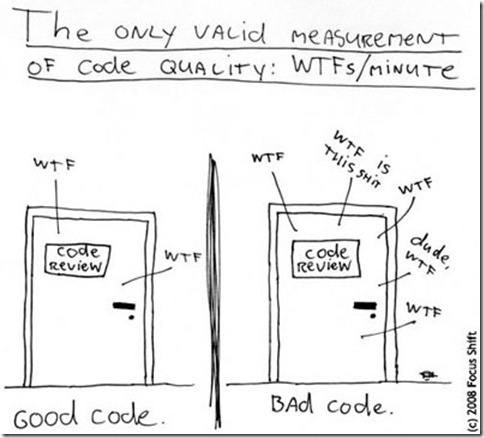
\includegraphics[height=.98\textheight]{content/chapter_testing/testing_intro/wtfs-minute}}}
}
\only<article>{\plain{\centerline{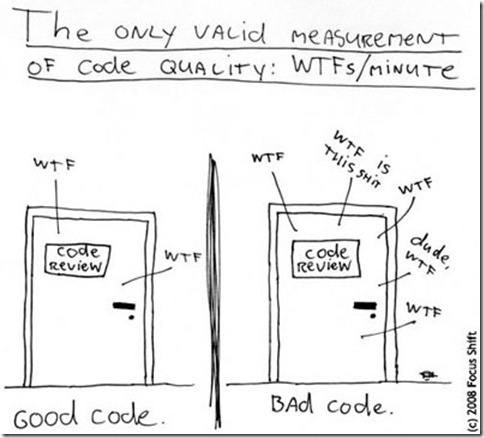
\includegraphics[width=\textwidth]{content/chapter_testing/testing_intro/wtfs-minute}}}\addtocounter{slidenumber}{1}}
\begin{Frame}{Human Unit Testing}
  \begin{itemize}
    \item Reading or visual inspection of a program by a\\
      \alert{team of people} (3-4 persons)
    \item Team includes other people than the programmer(s)
    \item Preparatory work \& conference
    \item Objective: find errors, but not solutions to the errors
    \item Two main techniques: \alert{inspections} and \alert{walkthroughs}
  \end{itemize}
\end{Frame}

\begin{Frame}{Terms}
  \inhead{Review} generic term\hfill\vspace{1ex}\linebreak
  \inhead{Manual review} no automation\hfill\vspace{1ex}\linebreak
  \inhead{Code review} review code, test cases, documentation\hfill\vspace{1ex}\linebreak
  \inhead{Technical review} review requirement documents, diagrams\hfill\vspace{1ex}\linebreak
  \inhead{Peer review} author and colleagues\hfill\vspace{1ex}\linebreak
  \inhead{Walkthrough} review code by playing computer\\
  (sometimes also: information exchange, brainstorming)\hfill\vspace{1ex}\linebreak
  \inhead{Pair programming} review during active development
\end{Frame}

\subsubsection*{Code Inspections}

\begin{Frame}{Code Inspections}
  \begin{itemize}
    \item A set of procedures and error-detection techniques for code reading
    \item Lots of literature on procedures, forms to be filled etc. (Perry, 2000)
    \item Disagreement with respect to whether a group meeting is necessary
    \item For group meeting (Myers, 1979), typically four people: a \alert{moderator}, the \alert{programmer},
    the \alert{program's designer} and a \alert{test specialist}
  \end{itemize}
\end{Frame}

\begin{Frame}{Typical Procedure for Code Inspections}
  \begin{itemize}
    \item The moderator distributes program and specification in advance
    to the other participants
    \item The programmer narrates the logic of the program (helps programmer to find errors)
    \item The program is analyzed with respect to a checklist of errors
    \item The programmer receives a list of the errors found, which is analyzed
    and used to refine the error checklist
    \item Advised length: 90--120 minutes
    \item About 150 lines per hour
  \end{itemize}
\end{Frame}

\begin{Frame}{An Error Checklist}
  \begin{itemize}
    \item sublist of the original list in (Myers, 1979)
    \item Progress in compiler and language design has made many items
    of the original list obsolete.
    \item List divided into \alert{data reference}, \alert{data declaration},
    \alert{computation}, \alert{comparison}, \alert{control-flow},
    \alert{interfaces}, and \alert{input/output} errors.
  \end{itemize}
\end{Frame}

\begin{Frame}{An Error Checklist}{Data Reference}
  \begin{itemize}
    \item Uninitialized variables used?
    \item Array indices within bounds?
    \item String limits exceeded?
    \item Dangling references?
    \item Correct types when aliasing?
    \item Off-by-one errors in indexing or subscripting operations?
  \end{itemize}
\end{Frame}

\begin{Frame}{An Error Checklist}{Data Declaration}
  \begin{itemize}
    \item All variables initialized?
    \item If not, default values understood?
    \item Arrays and strings initialized properly?
    \item All variables have the correct types?
    \item Any variables with similar names?
  \end{itemize}
\end{Frame}

\begin{Frame}{An Error Checklist}{Computation Errors}
  \begin{itemize}
    \item Mixed-mode computations (automatic conversions)?
    \item Intermediate result overflow or underflow?
    \item Division by zero?
    \item Operator precedence understood?
    \item Integer divisions correct?
    \item Variable's value outside of meaningful range?
  \end{itemize}
\end{Frame}

\begin{Frame}{An Error Checklist}{Comparison Errors}
  \begin{itemize}
    \item Comparison relationships correct?
    \item Boolean expressions correct?
    \item Operator precedence understood?
    \item Compiler evaluation of Boolean expressions understood?
  \end{itemize}
\end{Frame}

\begin{Frame}{An Error Checklist}{Control-flow Errors}
  \begin{itemize}
    \item Will each loop terminate?
    \item Will program terminate?
    \item Any loop bypasses because of entry conditions?
    \item Off-by-one iterations errors?
    \item Any non-exhaustive decisions?
  \end{itemize}
\end{Frame}

\begin{Frame}{An Error Checklist}{Interface Errors}
  \begin{itemize}
    \item Parameters and arguments match (number and order)?
    \item Number, attributes, and order of arguments to built-in functions correct?
  \end{itemize}
\end{Frame}

\begin{Frame}{An Error Checklist}{Input/ Output Errors}
  \begin{itemize}
    \item Format specification matches I/O statement?
    \item Buffer size matches record size?
    \item Files opened before use?
    \item End-of-file conditions handled?
    \item I/O errors handled?
    \item Any textual errors in output information?
  \end{itemize}
\end{Frame}

\begin{Frame}{An Error Checklist}{Other Checks}
  \begin{itemize}
    \item Any unreferenced variables in cross-reference listing?
    \item Any warning or informational messages?
    \item Input checked for validity?
    \item Missing function?
  \end{itemize}
\end{Frame}

\begin{Frame}[allowframebreaks]{An Error Checklist}{Some (Rather) Obsolete Errors}
  \begin{itemize}
    \item Computing addresses of bit strings? Passing bit-string arguments?
    \item Structure definitions match across procedures?
    \item All variables declared?
    \item Initialization consistent with storage class?
    \item Computations on non-arithmetic variables?
    \item Base-2 inaccuracies?
    \item Comparison and Boolean expressions mixed?
  \end{itemize}
  
  \framebreak

  \begin{itemize}
    \item Comparisons of base-2 fractional values?
    \item Do begin and end statements match?
    \item Number of arguments transmitted to called modules equal to number of parameters?
    \item Attributes of arguments transmitted to called modules equal to attributes of parameters?
    \item Units system of arguments transmitted to called modules equal to units system of parameters?
  \end{itemize}
\end{Frame}

\subsubsection*{Walkthroughs}

\begin{Frame}{Walkthroughs}
  General scheme similar to that of inspections, but:
  \begin{itemize}
    \item A member of the team acts as \alert{tester}.
    \item The tester comes to the meeting with some test cases.
    \item The participants \alert{play computer}, the current state of the program is monitored.
  \end{itemize}
\end{Frame}

\begin{Frame}{Empirical Data on Walkthroughs}
  \begin{itemize}
    \item Several studies available in the literature.
    \item Code distributed to some testers (small groups) in controlled situations.
    \item Code inspection finds between 30 and 50 \% of all errors.
  \end{itemize}
\end{Frame}

\subsubsection*{Social Effects}

\begin{Frame}[fragile]{Social Effects: Knowledge}
  Knowledge spreads through the team
  \begin{itemize}
    \item Experts and juniors share knowledge
    \item Real-time feedback for developers
    \item \alert{Responsibility} for entire project on whole team Maintaining not only depends on author
    \item Developers learn to spot errors and are more cautious New team members get to know the project
    \item Improve teamwork, because learning from each other becomes natural
  \end{itemize}
\end{Frame}

\begin{Frame}{Social Effects: Illusionary Confidence}
  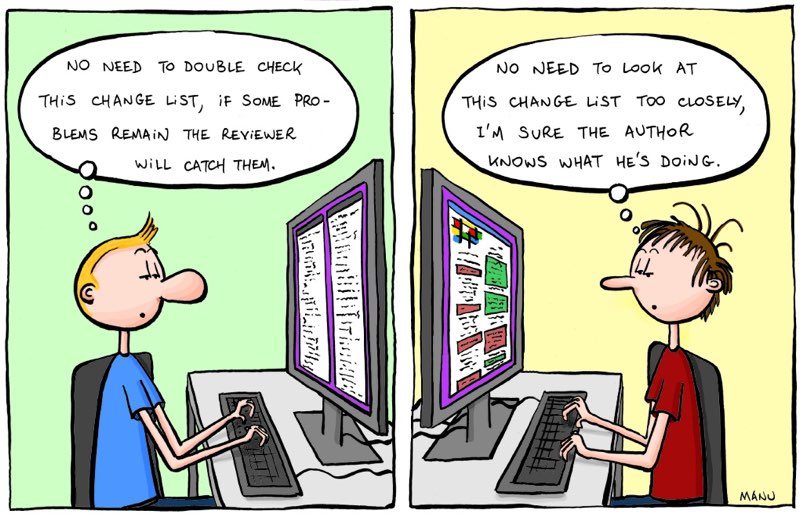
\includegraphics[width=\textwidth]{content/chapter_testing/testing_intro/confidence}

  \xxx

  \source{\href{http://www.bonkersworld.net/code-reviews}{www.bonkersworld.net/code-reviews}, December 1, 2013}
\end{Frame}

\begin{Frame}{Social Effects: Reputation}
  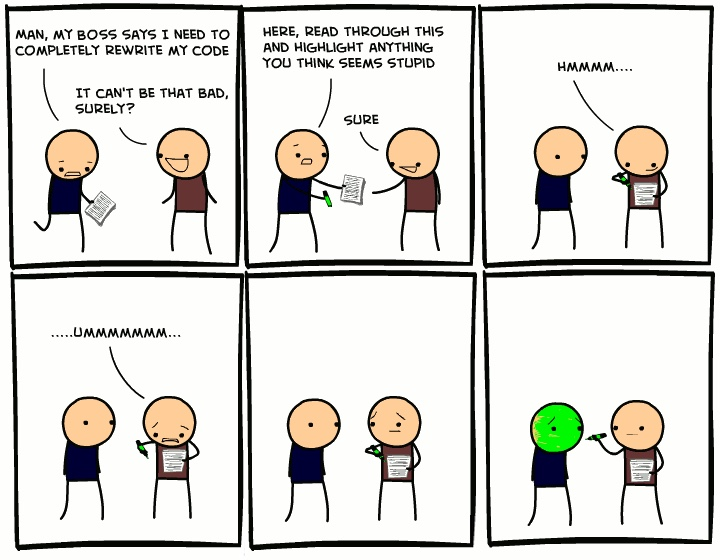
\includegraphics[width=\textwidth]{content/chapter_testing/testing_intro/reputation}

  \source{\href{http://blog.manishchhabra.com/2012/12/code-reviews-should-be-the-universal-rule-of-serious-software-development/}{blog.manishchhabra.com/2012/12/ code-reviews-should-be-the-universal-rule-of-serious-software-development/}, December 1, 2013}
\end{Frame}

\begin{Frame}{Social Effects}{Some Advices for Managers}
  \begin{itemize}
    \item Its about the code, not the person!
    \item Mix the code review team members.
    \item Explain to the team, that you \alert{want} them to find defects.
  \end{itemize}
\end{Frame}

\begin{Frame}{Social Effects}{Some Advices for Reviewers}
  \begin{itemize}
    \item Also point out good things!
    \item Be respectful, and patient.
    \item Everyone makes mistakes, even you.
    \item Learn from others, from their skills and\\
      from their mistakes.
    \item Avoid accusations, ask questions\\
      instead of making statements.
  \end{itemize}

  \xxx

  \source{Improve Quality and Morale: Tips for Managing the Social Effects of Code Review, SmartBear Software,
\href{http://support.smartbear.com/resources/cc/codereviewsocialeffects.pdf}{support.smartbear.com/resources/cc/codereviewsocialeffects.pdf}, June 15, 2014}
\end{Frame}





%!TEX root = ../../main.tex

\section{Conclusion}

\begin{frame}{Conclusion}
\begin{itemize}
\itemsep1em
\item Model Checking is an \hl{automatic} approach to \hl{verify} whether a given system satisfies a given specification
\item Proof of \hl{correctness} or \hl{counterexample} 
\item System properties: \hl{liveness, safety, invariants}
\item Symbolic Model Checking: make possible to handle infinite state systems and work around the state explosion problem
\item Over-/Under-approximation to abstract away superfluous information
\item Software Model Checking: no algorithm for all cases $\rightarrow$ combine different approaches    
\end{itemize}

\end{frame}



%\section{Black and White Boxes}

\scriptintro
\todoForMS{Write Intro}

\mode
<all>

\targets{
  \item Understand the different approaches of black- and white-box testing.
  \item Be able to compute equivalence partitions and boundary values.
  \item Be able to generate test cases based on path coverage.
  \item Know JUnit and EMMA.
}

\section{Black-Box Testing}

% Computer-assisted Unit Testing

\begin{Frame}{Computer-assisted Unit Testing}
  Test cases to be executed by a computer\\
  can have several levels of automation:

  \begin{itemize}
    \item Test suite generated \alert{manually}\\
      (still the most common case)
    \item Test suite generated \alert{manually with some tool assistance }
    \item Test suite generated \alert{automatically}\\
      (specific areas, mostly research)
  \end{itemize}
  
  \xxx

  \begin{description}
    \item[Black-box testing] \alert{no access} to source code,\\
      test cases designed solely \alert{from specification}
    \item[White-box testing] \alert{access} to source code,\\
      test cases designed \alert{from specification and code}
  \end{description}
\end{Frame}

\begin{Frame}{Methodologies to Design a Test Suite}
  \inhead{Black-box Testing}

  \begin{itemize}
    \item Equivalence partitioning
    \item Boundary-value analysis
  \end{itemize}

  \xxx

  \inhead{White-box Testing}

  \begin{itemize}
    \item Control-flow based path coverage
    \item Data-flow based path coverage
  \end{itemize}
\end{Frame}

\begin{Frame}{Methodologies to Design a Test Suite}{Black-box Testing}
  \begin{definition}[Equivalence Partitioning]
    Partition the \alert{input domain} of a program into a finite number of
    \alert{equivalence classes} such that one can \alert{reasonably assume} that a test of a representative value of each class is equivalent to a test of any other value.
  \end{definition}

  \xxx

  \begin{definition}[Boundary-value Analysis]
    Choose test cases directly \enquote{on}, \enquote{above}, and \enquote{beneath} the edges of equivalence classes.
  \end{definition}

  \xxx

  Usually applied together, boundary-value analysis used to add new test cases after equivalence partitioning.s
\end{Frame}


\subsection{Equivalence Partitioning}

\begin{Frame}{Equivalence Partitioning}{I. Identify the equivalence classes}
  \begin{itemize}
    \item Take \alert{each input condition} and partition it into
    \item at least one group of \alert{valid equivalence classes} and
    \item at least one group of \alert{invalid equivalence classes}.
  \end{itemize}

  \xxx

  \begin{example}
    \inhead{Input condition}\newline
    \enquote{$x$ is an integer between 0 and 100.}\hfill\vspace{1ex}\linebreak
    

    \inhead{Equivalence classes}
    \begin{itemize}
      \item $0 \ge x \ge 100$ (valid inputs)
      \item $x < 0$ (invalid inputs)
      \item $x > 100$ (invalid inputs)
    \end{itemize}
  \end{example}
\end{Frame}

\begin{Frame}{Equivalence Partitioning}{II. Define the test cases}
  \begin{enumerate}
    \item Assign a unique number to each equivalence class.
    \item Until all equivalence classes have been covered by test cases, write a new test case covering \alert{as many of the uncovered valid equivalence classes as possible}.
    \item Until all equivalence classes have been covered by test cases, write a new test case that covers \alert{one and only one of the uncovered invalid equivalence classes}.
    \end{enumerate}

    \xxx

    \begin{alertblock}{Why?}
      \pause
      \begin{itemize}
        \item Positive examples should \alert{cover many} valid equivalence classes to make the tests more complicated.
        \item Negative examples should \alert{cover one} invalid equivalence class to identify a specific bug when failing.
      \end{itemize}
    \end{alertblock}
\end{Frame}

\begin{Frame}[fragile]{\lstinline-mylogin- Example}
  Given a user ID and a password the function \lstinline-mylogin- checks whether the user can login.

  \begin{lstlisting}[language=Java,gobble=4]
    boolean mylogin(String userid,
                    String password);
  \end{lstlisting}

  \begin{itemize}
    \item \lstinline-userid- must be an alphanumeric string of length between 1 and 32 characters containing no numerical character before an alphabetic character.
    \item \lstinline-password- must be a string between 8 and 64 characters without blanks, with at least one numerical or special character, and different from \lstinline-userid-.
  \end{itemize}
\end{Frame}

\begin{Frame}[fragile]{Equivalence Classes}{\lstinline-mylogin- Example}
	\begin{center}
  \footnotesize\begin{zebratabular}{p{3.3cm}p{2.1cm}p{3.3cm}}
  \headerrow input condition & Valid eq. class & invalid eq. class \\
  \lstinline-userid- is alphanumeric & yes (1) & no (2) \\
  $1 \le |\text{\lstinline-userid-}| \le 32$ & yes (3) & 
  $|\text{\lstinline-userid-}|< 1$ (4), \newline
  $|\text{\lstinline-userid-}|>32$ (5) \\
  no num. before alph. & yes (6) & 
  all char. numeric (7), \newline
  num. char. followed\newline by alph. char. (8)\\
  $8 \le |\text{\lstinline-password-}| \le 64$ & yes (9) & 
  $|\text{\lstinline-password-}|< 8$ (10), \newline
  $|\text{\lstinline-password-}|> 64$ (11)\\
  no blanks & yes (12) & no (13) \\
  one num. or sp. char. & 
  yes, num. (14), \newline
  yes, sp. (15) & no (16) \\
  diff. from \lstinline-userid- & yes (17) & no (18) \\
  \end{zebratabular}
  \end{center}
\end{Frame}

\begin{Frame}[fragile]{Test Cases}{\lstinline-mylogin- Example}
	\begin{center}
  \begin{zebratabular}{llllp{2cm}}
    \headerrow \# & userid &  password  & result & eq. classes \\
    1 & \texttt{leucker} & \texttt{leucker0} & accept & 1,3,6,9, 12,14,17 \\
    2 & \texttt{leucker} & \texttt{leucker!} & accept & 1,3,6,9, 12,15,17 \\
    3 & \texttt{leucker?} & \texttt{leucker!} & reject & 2 \\
    4 & \textit{empty} & \texttt{leucker!} & reject & 4 \\
    5 & \texttt{l$^{27}$eucker} & \texttt{leucker!} & reject & 5 \\
    6 & \texttt{7546} & \texttt{leucker!} & reject & 7 \\
    7 & \texttt{le5ucker} & \texttt{leucker!} & reject & 8 \\
    8 & \texttt{leucker} & \texttt{leucke0} & reject & 10 \\
    9 & \texttt{leucker} & \texttt{l$^{58}$eucker0} & reject & 11 \\
    10 & \texttt{leucker} & \lstinline[showspaces=true,identifierstyle={}]-leuc ker0- & reject & 13 \\
    11 & \texttt{leucker} & \texttt{lleucker} & reject & 16 \\
    12 & \texttt{leucker0} & \texttt{leucker0} & reject & 18 \\
  \end{zebratabular}
  \end{center} 
\end{Frame}

\subsection*{Boundary Values}

\begin{frame}{Boundary Values}
  \textcolor{maincolor}{Differs from equivalence partitioning in two respects:}

  \begin{itemize}
    \item Instead of selecting any element of an equivalence class, one or
      more elements are selected such that each \enquote{edge} of the equivalence class
      is the subject of a test.
    \item Test cases are also derived by considering the \alert{result space};
      i.e., output equivalence classes.
  \end{itemize} 
\end{frame}

\begin{Frame}{Boundary Values}{Some Guidelines}
  \begin{itemize}
    \item If an input condition specifies a range of values, write test cases for the ends of the range, and invalid-input test cases for situations just beyond the ends.
    \item If an output condition specifies a range of values, write test cases for the ends of the range, and see if there might be cases causing an output beyond the ends.
    \item If the input or output is an ordered set (array, string, list, table, \ldots) focus attention on the first and last elements of the set.
    \item Use your ingenuity to search for other boundary conditions.
  \end{itemize}
\end{Frame}

\begin{Frame}[allowframebreaks,fragile]{Test Cases From Boundary Values}{\lstinline-mylogin- Example}
  Write a test case in which all characters of \lstinline-userid- are alphanumeric.\hfill\vspace{1ex}\linebreak

  \begin{zebratabular}{llllp{2cm}}
    \headerrow \# & userid &  password  & result & eq. classes \\
    1 & \texttt{leucker} & \texttt{leucker0} & accept & 1,3,6,9, 12,14,17 \\
  \end{zebratabular}

  \framebreak

  Write test cases in which the first, the last, all characters of
  \lstinline-userid- are not alphanumeric.\hfill\vspace{1ex}\linebreak

  \begin{zebratabular}{llllp{2cm}}
    \headerrow \# & userid &  password  & result & eq. classes \\
    3 & \texttt{leucker?} & \texttt{leucker!} & reject & 2 \\
    13 & \texttt{!leucker} & \texttt{leucker0} & reject & \textcolor{alertedcolor}{new} \\
    14 & \texttt{!!!}  & \texttt{leucker0} & reject & \textcolor{alertedcolor}{new} \\
  \end{zebratabular}

  \framebreak

  Write test cases where \lstinline-userid- has length 0, 1, 32, and 33.\hfill\vspace{1ex}\linebreak

  \begin{zebratabular}{llllp{2cm}}
    \headerrow \# & userid &  password  & result & eq. classes \\
    4 & \textit{empty} & \texttt{leucker!} & reject & 4 \\
    5 & \texttt{l$^{27}$eucker} & \texttt{leucker!} & reject & 5 \\
    15 & \texttt{l} & \texttt{leucker0} & accept & \textcolor{alertedcolor}{new} \\
    16 & \texttt{l$^{26}$eucker} & \texttt{leucker0} & accept & \textcolor{alertedcolor}{new} \\
  \end{zebratabular}

  \framebreak

  Write a test case in which the first character of \lstinline-userid-
  is alphabetic and all others numeric.\hfill\vspace{1ex}\linebreak

  \begin{zebratabular}{llllp{2cm}}
    \headerrow \# & userid &  password  & result & eq. classes \\
    17 & \texttt{l1234} & \texttt{leucker0} & accept & \textcolor{alertedcolor}{new} \\
  \end{zebratabular}

  \framebreak

  Write test cases in which\\
  \ \ -- the first character of \lstinline-userid- is numerical,\\
  \ \ -- the last two characters are numeric-alphabetic,\\
  \ \ -- all characters are numeric.\hfill\vspace{1ex}\linebreak

  \begin{zebratabular}{llllp{2cm}}
    \headerrow \# & userid &  password  & result & eq. classes \\
    6 & \texttt{7546} & \texttt{leucker!} & reject & 7 \\
    18 & \texttt{1leucker} & \texttt{leucker0} & reject & \textcolor{alertedcolor}{new} \\
    19 & \texttt{leuc0r} & \texttt{leucker0} & accept & \textcolor{alertedcolor}{new} \\
  \end{zebratabular} 

  \framebreak

  Write test cases where \lstinline-password- has length 7, 8, 64, and 65.\hfill\vspace{1ex}\linebreak

  \begin{zebratabular}{llllp{2cm}}
    \headerrow \# & userid &  password  & result & eq. classes \\
    1 & \texttt{leucker} & \texttt{leucker0} & accept & 1,3,6,9, 12,14,17 \\
    8 & \texttt{leucker} & \texttt{leucke0} & reject & 10 \\
    9 & \texttt{leucker} & \texttt{l$^{58}$eucker0} & reject & 11 \\
    21 & \texttt{leucker} & \texttt{l$^{57}$eucker0} & accept & \textcolor{alertedcolor}{new} 
  \end{zebratabular}

  \framebreak

  Write a test case in which \lstinline-password- contains no blanks.\hfill\vspace{1ex}\linebreak

  \begin{zebratabular}{llllp{2cm}}
    \headerrow \# & userid &  password  & result & eq. classes \\
    1 & \texttt{leucker} & \texttt{leucker0} & accept & 1,3,6,9, 12,14,17 \\
  \end{zebratabular}

  \framebreak

  Write test cases in which the first, the last, all characters of
  \lstinline-password- are blanks.\hfill\vspace{1ex}\linebreak

  \begin{zebratabular}{llllp{2cm}}
    \headerrow \# & userid &  password  & result & eq. classes \\
    22 & \texttt{leucker} & \lstinline[showspaces=true,identifierstyle={}]- leucker- & reject & \textcolor{alertedcolor}{new} \\
    23 & \texttt{leucker} & \lstinline[showspaces=true,identifierstyle={}]-leucker - & reject & \textcolor{alertedcolor}{new} \\
    24 & \texttt{leucker} & \lstinline[showspaces=true,identifierstyle={}]-   - & reject & \textcolor{alertedcolor}{new} \\
  \end{zebratabular}

  \framebreak

  Write a test case in which just the first or the last character of
  \lstinline-password- is numeric.\hfill\vspace{1ex}\linebreak

  \begin{zebratabular}{llllp{2cm}}
    \headerrow \# & userid &  password  & result & eq. classes \\
    1 & \texttt{leucker} & \texttt{leucker0} & accept & 1,3,6,9, 12,14,17 \\
    25 & \texttt{leucker} & \texttt{0leucker} & reject & \textcolor{alertedcolor}{new} \\
  \end{zebratabular} 

  \framebreak

  Write a test case in which just the first or the last character 
  of \lstinline-password- is special.\hfill\vspace{1ex}\linebreak

  \begin{zebratabular}{llllp{2cm}}
    \headerrow \# & userid &  password  & result & eq. classes \\
    2 & \texttt{leucker} & \texttt{leucker!} & accept & 1,3,6,9, 12,15,17 \\
    26 & \texttt{leucker} & \texttt{!leucker} & reject & \textcolor{alertedcolor}{new} \\
  \end{zebratabular} 

  \framebreak

  Write a test case in which \lstinline-password-
  has no numeric or special characters.\hfill\vspace{1ex}\linebreak

  \begin{zebratabular}{llllp{2cm}}
    \headerrow \# & userid &  password  & result & eq. classes \\
    11 & \texttt{leucker} & \texttt{lleucker} & reject & 16 \\
  \end{zebratabular} 
\end{Frame}

\subsection{MTEST example}

\begin{Frame}{The MTEST example}{Specification of input I}
  MTEST is a program that grades multiple-choice examinations. The input is a file named OCR, which contains 80-character records. The first record is a title; the contents of this record are used as a title on each output report. The next set of records describes the correct answers on the exam. Each record contains a 2 as the last character. In the first record of this set, the number of questions is listed in columns 1--3 (a value of 1--999). Columns 10--59 contain the correct answers for questions 1--50 (any character is valid as an answer). Subsequent records contain, in columns 10--59, the correct answers for questions 51--100, 101--150, and so on.
\end{Frame}

\begin{Frame}{The MTEST example}{Specification of input II}
  The third set of records describes the answers of each student; each record contains a 3 in column 80. For each student, the first record contains the student's name or number in columns 1--9 (any characters); columns 10--59 contain the student's answers for questions 1--50. If the test has more than 50 questions, subsequent records for the student contain answers 51--100, 101--150, and so on, in columns 10--59. The maximum number of students is 200. 
\end{Frame}

\begin{Frame}{The MTEST example}{Specification of output}
  The four output records are 
  \begin{itemize}
    \item[(1)] a report, sorted by student identifier, showing each student's grade (percentage of answers correct) and rank; 
    \item[(2)] a similar report, but sorted by grade;  
    \item[(3)] a report indicating the mean, median, and standard deviation of the grades; and 
    \item[(4)] a report, ordered by question number, showing the percentage of students answering each questions correctly.
  \end{itemize}
\end{Frame}

\begin{Frame}{Test cases from input conditions I}
  \begin{itemize}
    \item[1.] Empty input file
    \item[2.] Missing title record
    \item[3.] 1-character title
    \item[4.] 80-character title
    \item[5.] 0-question exam
    \item[6.] 1-question exam
    \item[7.] 50-question exam
    \item[8.] 51-question exam
    \item[9.] 999-question exam
    \item[10.] Number-of-questions field has non-numeric value
  \end{itemize}
\end{Frame}

\begin{Frame}{Test cases from input conditions II}
  \begin{itemize}
    \item[11.] No correct-answer records after title record
    \item[12.] One too many correct-answer records
    \item[13.] One too few correct-answer records
    \item[14.] 0 students
    \item[15.] 1 student
    \item[16.] 200 students
    \item[17.] 201 students
  \end{itemize}
\end{Frame}

\begin{Frame}{Test cases from input conditions III}
  \begin{itemize}
    \item[18.] A student has one answer record, but there are two correct-answer records.
    \item[19.] The above student is the first student in the file.
    \item[20.] The above student is the last student in the file.
    \item[21.] A student has two answer records, but there is just one correct-answer record.
    \item[22.] The above student is the first student in the file.
    \item[23.] The above student is the last student in the file.
  \end{itemize}
\end{Frame}

\begin{Frame}{Test cases from output conditions}{Reports 1 and 2}
  \begin{itemize}
    \item 0, 1, 200  students (same as test 14,15,16)
    \item[24.] All students receive the same grade.
    \item[25.] All students receive a different grade.
    \item[26.] Some, but not all, students receive the same grade (to see if ranks are computed correctly).
    \item[27.] A student receives a grade of 0.
    \item[28.] A student receives a grade of 100.
    \item[29.] A student has the lowest possible identifier value (to check the sort).
    \item[30.] A student has the highest possible identifier value.
    \item[31.] The number of students is such that the report is just large enough to fit on one page (to see if an extraneous page is printed).
    \item[32.] The number of students is such that all students but one fit on one page
  \end{itemize}
\end{Frame}

\begin{Frame}{Test cases from output conditions}{Report 3}
  \begin{itemize}
    \item[33.] The mean is at its maximum (all students have a perfect score)
    \item[34.] The mean is 0 (all students receive a grade of 0)
    \item[35.] The standard deviation is at its maximum (one student receives a 0 and the other receives a 100).
    \item[36.] The standard deviation is 0 (all students receive the same grade).
  \end{itemize}
\end{Frame}

\begin{Frame}{Test cases from output conditions}{Report 4}
  \begin{itemize}
    \item[37.] All students answer question 1 correctly.
    \item[38.] All students answer question 1 incorrectly.
    \item[39.] All students answer the last question correctly.
    \item[40.] All students answer the last question incorrectly.
    \item[41.] The number of questions is such that the report is just large enough to fit on one page.
    \item[42.] The number of questions is such that all questions but one fit on one page.
  \end{itemize}
\end{Frame} %MTEST as exercise?

\subsection*{JUnit \& EMMA}

\begin{Frame}{Unit Testing in Practice}
  \begin{itemize}
    \item Most methodologies for unit testing, the rest rather ad-hoc (but see later).
    \item Unit testing often done by the programmer.
  \end{itemize}

  \inhead{Popular Procedure for Self-testing}
  \begin{enumerate}
    \item Use a black-box technique to generate\\
      a first set of test cases.
    \item Use a tool to compute the degree of coverage and\\
      the statements/edges/conditions/multiple conditions\\
      not yet covered.
    \item Add new test cases to provide full coverage or\\
      a degree of coverage considered adequate.
    \item The module can only be delivered for integration\\
      together with the (successfully passed) test cases.
  \end{enumerate}
\end{Frame}



\subsubsection*{JUnit}

\begin{frame}{JUnit}
  \begin{itemize}
    \item Unit testing framework for Java
    \item Developed by Erich Gamma and Kent Beck
    \item Current version: JUnit 5.x 
    \item Download: Comes with Eclipse or at \href{http://www.junit.org}{www.junit.org}
    \item Goal: Simplify the definition of test cases (as Java code) and the execution of test cases for Java.
  \end{itemize} 
\end{frame}

\begin{Frame}[fragile]{Simple Test Case (Beck \& Gamma)}
  \begin{itemize}
    \item Annotate a method with \lstinline[language=Java]-@org.junit.Test-.
    \item When you want to check a value
      \begin{lstlisting}[language=java,gobble=8]
        import static org.junit.Assert.*;
      \end{lstlisting}
    \item Call \lstinline[language=Java]-assertTrue();- and pass a boolean that is true if the test succeeds.
  \end{itemize}

  \xxx

  \begin{lstlisting}[language=java,gobble=4]
    @Test
    public void simpleAdd() {
      Money m12CHF = new Money(12, "CHF"); 
      Money m14CHF = new Money(14, "CHF"); 
      Money expected = new Money(26, "CHF"); 
      Money result = m12CHF.add(m14CHF); 
      assertTrue("Money should add up",
        expected.equals(result));
    }
  \end{lstlisting}
\end{Frame}

\begin{Frame}[allowframebreaks,fragile]{Other Assertion Statements}
  Without any assertion a test always passes.

  \xxx

  \begin{lstlisting}[language=Java,gobble=4]
    fail(String message);
  \end{lstlisting}
  Let the test case fail with the given message.

  \xxx

  \begin{lstlisting}[language=Java,gobble=4]
    assertEquals(String message,
      expected, actual);
  \end{lstlisting}

  Test if the values are the same. Note: for arrays the reference is checked not the content of the arrays.

  \xxx

  \begin{lstlisting}[language=Java,gobble=4]
    assertArrayEquals(String message,
      expecteds, actuals);
  \end{lstlisting}

  Test if the given arrays contain the same values.

  \framebreak

  \begin{lstlisting}[language=Java,gobble=4]
    assertEquals(String message,
      expected, actual, tolerance);
  \end{lstlisting}

  Usage for float and double; the tolerance are the number of decimals which must be the same.

  \xxx

  \begin{lstlisting}[language=Java,gobble=4]
    assertNull(String message, object);
  \end{lstlisting}

  Test of an object reference is null.

  \xxx

  \begin{lstlisting}[language=Java,gobble=4]
    assertSame(String message,
      expected, actual);
  \end{lstlisting}

  Test if the given object references point to the some object.

  \framebreak

  \begin{lstlisting}[language=Java,gobble=4]
    assertTrue(String message,
      boolean condition);
  \end{lstlisting}

  Test if the boolean condition holds. Avoid usage if any other assertion is more specific.
\end{Frame}

\begin{Frame}{Fixture (Beck \& Gamma)}
  How to write many test cases for operating within the same
    environment/setup/\alert{fixture}?
  \begin{enumerate}
    \item Add a field for each part of the fixture.
    \item Annotate a method with \lstinline[language=java]-@org.junit.Before- and initialize the variables in that method.
    \item Annotate a method with \lstinline[language=java]-@org.junit.After- to release any permanent resources you allocated in setup.
  \end{enumerate}
\end{Frame}

\begin{Frame}[fragile]{Fixture (Beck \& Gamma)}{Example}
  \begin{lstlisting}[language=java,gobble=4]
    public class MoneyTest { 
      private Money f12CHF; 
      private Money f14CHF; 
      private Money f28USD; 
    
      @Before
      public void setUp() { 
        f12CHF = new Money(12, "CHF"); 
        f14CHF = new Money(14, "CHF"); 
        f28USD = new Money(28, "USD"); 
      }
    }
  \end{lstlisting}
\end{Frame}

\begin{Frame}[fragile]{Running Tests (Beck \& Gamma)}
  \begin{itemize}
    \item Run from a Java program:
      \begin{lstlisting}[language=java,gobble=8]
        org.junit.runner.JUnitCore.
          runClasses(TestClass1.class,...);
      \end{lstlisting}
    \item Run from the command line:
      \begin{lstlisting}[language={},gobble=8]
        java org.junit.runner.JUnitCore \
          TestClass1 [...other test classes...]
      \end{lstlisting}
      with both your test class and junit on the classpath.
    \item Run from the command line using maven:
      \begin{lstlisting}[language={},gobble=8]
        mvn test -Dtest=TestClass1
      \end{lstlisting}
      Leave out the \lstinline[language={}]=-Dtest= option to run all tests.
  \end{itemize}
\end{Frame}

\begin{Frame}[fragile]{Expected Exception (Beck \& Gamma)}
  \begin{lstlisting}[language=java,gobble=4]
    new ArrayList<Object>().get(0);
  \end{lstlisting}
  should throw \lstinline[language=java]-IndexOutOfBoundsException-

  \xxx

  \begin{lstlisting}[language=java,gobble=4]
    @Test(expected=
      IndexOutOfBoundsException.class)
    public void empty() { 
      new ArrayList<Object>().get(0); 
    }
  \end{lstlisting}
\end{Frame}

\begin{Frame}{Other Annotations}
  \begin{itemize}
    \item \lstinline[language=java]-@BeforeClass- performs the method before the start of all tests. This can be used to perform time intensive activities, e.g. connect to a database.
    \item \lstinline[language=java]-@AfterClass- performs the method after all tests have finished. This can be used to perform clean-up activities, e.g. disconnect from a database.
    \item \lstinline[language=java]-@Ignore- ignores the test method, e.g. useful if the underlying code has been changed and the test has not yet been adapted or if the runtime of this test is just to long to be included.
    \item \lstinline[language=java]-@Test(timeout=100)- fails if the method takes longer then 100 milliseconds.
  \end{itemize}
\end{Frame}

\begin{frame}{Testing Frameworks}
Testing frameworks exist for most programming languages, for example
\begin{itemize}
	\item JUnit for Java
	\item Scalatest for Scala
	\item Check, cUnit and many more for C
	\item ...
\end{itemize}
\end{frame}

\subsubsection*{Checking Coverage with EMMA}

\begin{frame}[fragile]{Checking Coverage with EMMA}
  \begin{itemize}
    \item EMMA: \href{http://emma.sourceforge.net/}{emma.sourceforge.net}
    \item Run EMMA on the command line:
      \begin{lstlisting}[language={},gobble=8]
        java -cp emma.jar emmarun -jar \
          YourApp.jar
      \end{lstlisting}
      Insert \texttt{emmarun} between the JVM and your application.
    \item Run EMMA in Eclipse:\\
      Install EclEmma through the Eclipse Marketplace.
  \end{itemize}
\end{frame}

\begin{Frame}{Checking Coverage with EMMA}{Install EclEmma in Eclipse}
  \begin{center}
	  \only<presentation>{%
	    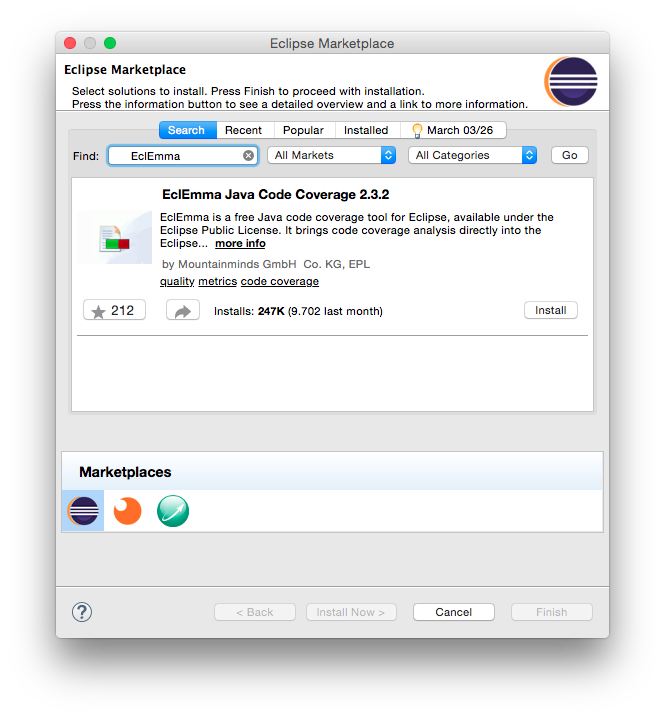
\includegraphics[height=.9\textheight]{content/chapter_testing/black+white/emma-eclipse-marketplace}
    }%
    \only<article>{%
	    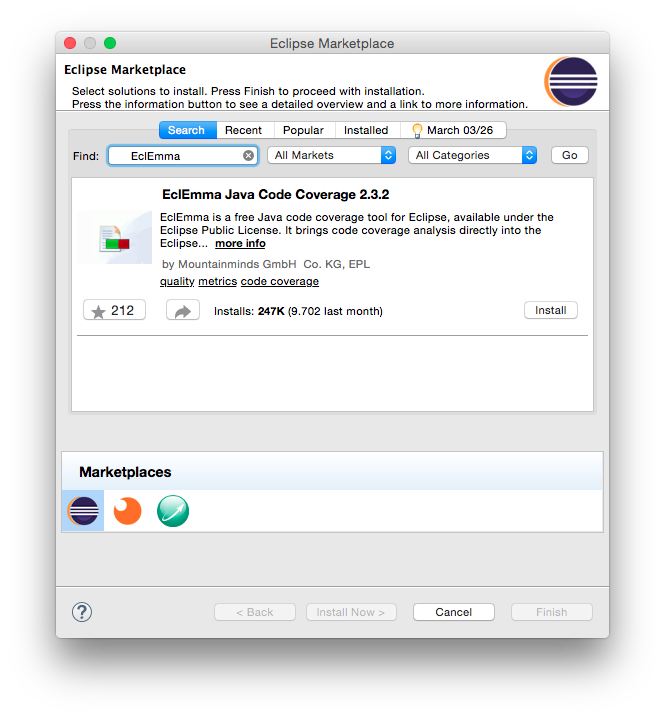
\includegraphics[width=\textwidth]{content/chapter_testing/black+white/emma-eclipse-marketplace}
    }%
  \end{center}
\end{Frame}

\subsubsection*{Triangle Example}

\begin{frame}{Recall the Triangle Exercise (Myers)}
  \begin{itemize}
    \item Input: three integer values\\
      representing lengths of the sides of a triangle.
    \item Output: \texttt{scalene}, \texttt{isosceles}, or \texttt{equilateral}
  \end{itemize}

  \xxx

  \hfill
  \shortstack{
    \tikz[auto,scale=.5]{
      \draw[draw=maincolor, thick]
        (0,0) -- node {4} ++(-4,0) -- node{3} ++(0,3) coordinate (last) -- cycle;
      \path (last) -- node{5} (0,0);}\\
    \texttt{scalene}\strut\\
    \scriptsize (unregelmäßig)
  }
  \hfill
  \shortstack{
    \tikz[auto,scale=.5]{
      \draw[draw=maincolor, thick]
        (0,0) -- node {3} ++(2,2.2361) -- node{3} ++(2,-2.2361) coordinate (last) -- cycle;
      \path (last) -- node{4} (0,0);}\\
    \texttt{isosceles}\strut\\
    \scriptsize (gleichschenklig)
  }
  \hfill
  \shortstack{
    \tikz[auto,scale=.5]{
      \draw[draw=maincolor, thick]
        (0,0) -- node {4} ++(2,3.4641) -- node{4} ++(2,-3.4641) coordinate (last) -- cycle;
      \path (last) -- node{4} (0,0);}\\
    \texttt{equilateral}\strut\\
    \scriptsize (gleichseitig)
  }
  \hfill\strut
\end{frame}

\begin{Frame}[fragile]{Write Java Skeleton}
  \begin{lstlisting}[language=java,gobble=4,basicstyle=\ttfamily\footnotesize]
    public class Triangle {
      public static enum Type {
        SCALENE, ISOSCELES, EQUILITERAL, INVALID;
      }
      
      public static Type getType(int a, int b, int c) {
        // TODO: implement
        throw new UnsupportedOperationException();
      }
    }
  \end{lstlisting}
\end{Frame}

\begin{Frame}[fragile,allowframebreaks]{Write Test Cases}
  \begin{lstlisting}[language=java,gobble=4,basicstyle=\ttfamily\footnotesize]
    @Test
    public void validScalene() {
      assertEquals(SCALENE, getType(2, 3, 4));
    }
    @Test
    public void validEquiliteral() {
      assertEquals(EQUILITERAL, getType(3, 3, 3));
    }
    @Test
    public void validIsoscelesAB() {
      assertEquals(ISOSCELES, getType(3, 3, 5));
    }
    @Test
    public void validIsoscelesAC() {
      assertEquals(ISOSCELES, getType(3, 5, 3));
    }
    @Test
    public void validIsoscelesBC() {
      assertEquals(ISOSCELES, getType(5, 3, 3));
    }
  \end{lstlisting}

  \framebreak

  \begin{lstlisting}[language=java,gobble=4,basicstyle=\ttfamily\footnotesize]
    @Test
    public void invalidZero() {
      assertEquals(INVALID, getType(0, 3, 3));
    }
    @Test
    public void invalidNegative() {
      assertEquals(INVALID, getType(-2, 3, 4));
    }
    @Test
    public void invalidNoAreaAB() {
      assertEquals(INVALID, getType(3, 3, 6));
    }
    @Test
    public void invalidNoAreaAC() {
      assertEquals(INVALID, getType(3, 6, 3));
    }
    @Test
    public void invalidNoAreaBC() {
      assertEquals(INVALID, getType(6, 3, 3));
    }
  \end{lstlisting}

	\framebreak

  \begin{lstlisting}[language=java,gobble=4,basicstyle=\ttfamily\footnotesize]
    @Test
    public void invalidTooLongA() {
      assertEquals(INVALID, getType(4, 2, 1));
    }
    @Test
    public void invalidTooLongB() {
      assertEquals(INVALID, getType(2, 4, 1));
    }
    @Test
    public void invalidTooLongC() {
      assertEquals(INVALID, getType(1, 2, 4));
    }
    @Test
    public void invalidZeros() {
      assertEquals(INVALID, getType(0, 0, 0));
    }
  \end{lstlisting}
\end{Frame}

\begin{Frame}{Run Test Cases}
  \begin{center}
    \only<presentation>{%
	    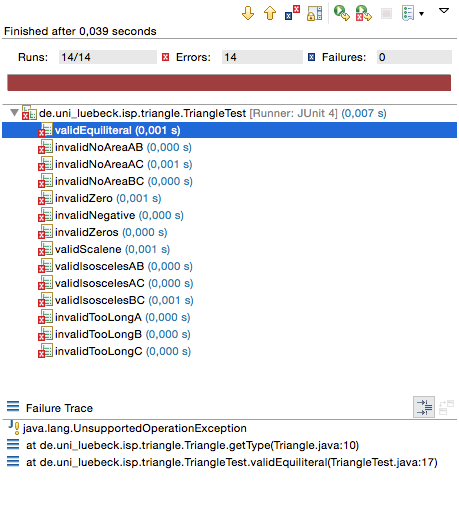
\includegraphics[height=.9\textheight]{content/chapter_testing/black+white/junit-fail}
    }%
    \only<article>{%
	    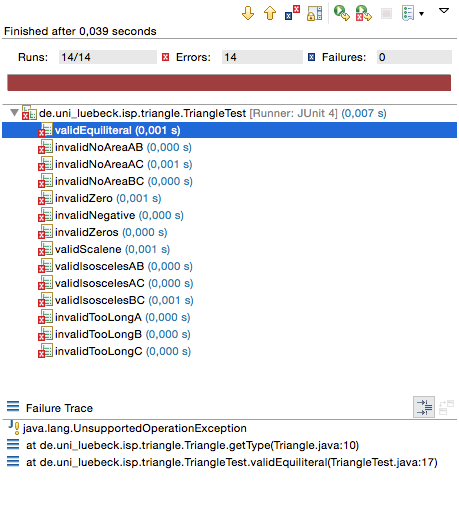
\includegraphics[width=\textwidth]{content/chapter_testing/black+white/junit-fail}
    }%
  \end{center}
\end{Frame}

\begin{Frame}[fragile]{Implement Method}
  \begin{lstlisting}[language=java,gobble=4,basicstyle=\ttfamily\footnotesize]
    public static Type getType(int a, int b, int c) {
      if (a <= 0 || b <= 0)
        return INVALID;
      if (abs(a) + abs(b) <= abs(c))
        return INVALID;
      if (abs(a) + abs(c) <= abs(b))
        return INVALID;
      if (abs(b) + abs(c) <= abs(a))
        return INVALID;
      if (a == b && b == c)
        return EQUILITERAL;
      if (a == b || b == c || a == c)
        return ISOSCELES;
      return SCALENE;
    }
  \end{lstlisting}
\end{Frame}

\begin{Frame}{Run Test Cases Again}
  \begin{center}
	  \only<presentation>{%
	    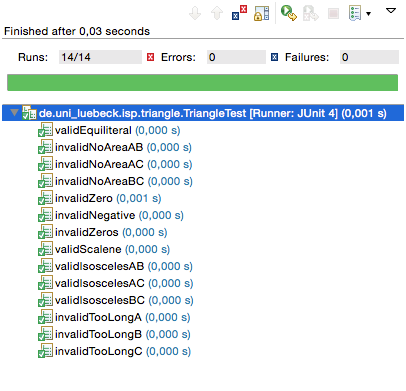
\includegraphics[height=.9\textheight]{content/chapter_testing/black+white/junit-pass}
    }%
    \only<article>{%
    	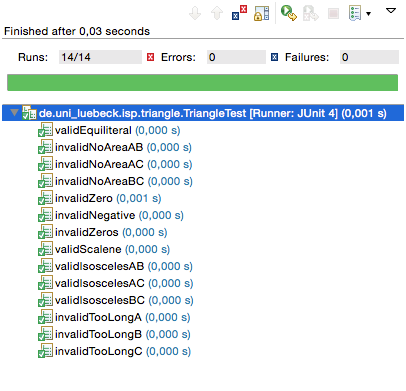
\includegraphics[width=\textwidth]{content/chapter_testing/black+white/junit-pass}
    }%
  \end{center}
\end{Frame}

\begin{Frame}{Run Coverage}
  \begin{center}
    \only<presentation>{%
	    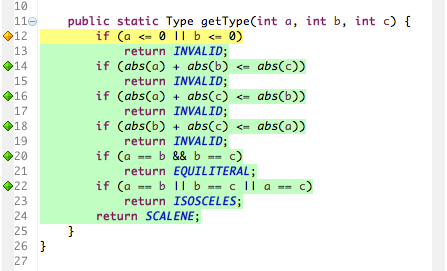
\includegraphics[width=.9\textheight]{content/chapter_testing/black+white/emma-fail}
    }%
    \only<article>{%
      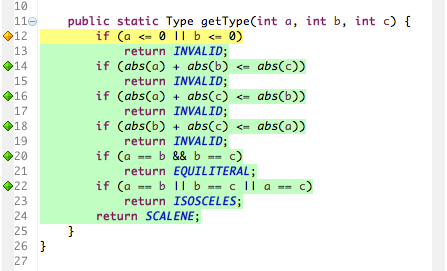
\includegraphics[width=\textwidth]{content/chapter_testing/black+white/emma-fail}
    }%
  \end{center}

  \xxx

  Negative values not completely tested.
\end{Frame}

\begin{Frame}[fragile]{Add More Test Cases}
  \begin{lstlisting}[language=java,gobble=4,basicstyle=\ttfamily\footnotesize]
    @Test
    public void invalidNegativeA() {
      assertEquals(INVALID, getType(-2, 3, 4));
    }
    @Test
    public void invalidNegativeB() {
      assertEquals(INVALID, getType(3, -2, 4));
    }
    @Test
    public void invalidNegativeC() {
      assertEquals(INVALID, getType(3, 4, -2));
    }
  \end{lstlisting}

  \xxx

  Only test case \lstinline[language=java]-invalidNegativeA- was already present.
\end{Frame}

\begin{Frame}{Run Test Cases Again}
  \centerline{
    \only<presentation>{%
      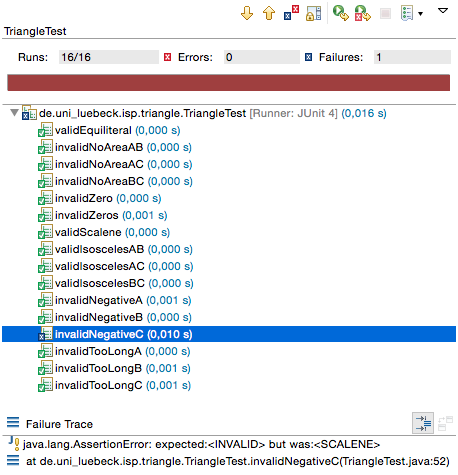
\includegraphics[height=.8\textheight]{content/chapter_testing/black+white/junit-bug}
    }%
    \only<article>{%
      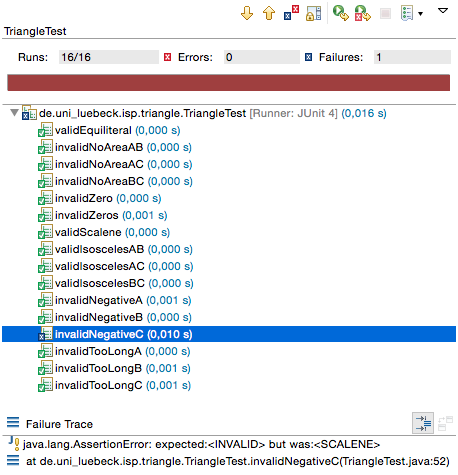
\includegraphics[width=\textwidth]{content/chapter_testing/black+white/junit-bug}
    }%
  }

  We found a bug.
\end{Frame}

\begin{Frame}[fragile]{Fix Implemented Method}
  \begin{lstlisting}[language=java,gobble=4,escapechar=/]
    if (a <= 0 || b <= 0/\alert{\texttt{ || c <= 0}}/)
      return INVALID;
  \end{lstlisting}

  \xxx

  \begin{LARGE}
    Now the test cases pass and\\
    cover the whole implementation.
  \end{LARGE}
\end{Frame}


\tikzset{%
	every state/.style={
		draw=maincolor,
		thick,
		fill=maincolor!18,
		inner sep=.8ex,
		minimum size=0pt
	},	
	field/.style={
		state,
		shape aspect=5,
		shape=rectangle
	},
	success/.style={
		state,
		field,
		fill=green!60!black!50
	},
	error/.style={
		state,
		field,
		fill=purple!50
	},
	shorten >=1pt,
	initial text={}
}

\section{Test-Driven Development (TDD)}


\subsection*{An Overview}

\begin{frame}{Test-Driven Development}
\begin{itemize}
	\item Waterfall or V-Model propose to write tests after the code which is tested with them.
	\item TDD proposes to write tests first, alternating with actual code
	\item Often found in agile development methods
	\item Tries to eliminate disadvantages of white-box testing and not sufficient test coverage
	\item TDD as presented in this section is mainly for unit tests. For system tests it can be used in the same way. Write or at least specify the system test before programming the system
\end{itemize}
\end{frame}

\begin{frame}{Using Test-Driven Development}
\begin{itemize}
	\item Write tests before the code they test is written.
	\item All such tests fail at first but should be fulfilled when the code is written.
	\item The same person can write tests and code.
\end{itemize}
\end{frame}

\begin{frame}{Tool Support for Test-Driven Development}
\begin{itemize}
	\item Tool for writing tests and automatic test execution (for Java: JUnit)
	\item Tool automatically building the project (Java: Ant, Maven, Gradle, ...)
\end{itemize}
\end{frame}

\subsection*{TDD by Kent Beck}

\begin{frame}{Test-Driven Development (Kent Beck)}
\begin{itemize}
	\item TDD done in micro steps (iterations)
	\item Write a unit test, implement that unit (one iteration)
	\item Write another unit test, change the written code to also fulfil this test (next iteration)
	\item Repeat this iterations until every case is covered. Each iteration should only take minutes.
	\item Each iteration has three steps:
	\begin{itemize}
		\item Write a test that tests a new behaviour. You should start with the easiest test case left. This test should fail.
		\item Change the code with as least effort as possible. So solve exactly the wanted case. The written test should be fulfilled now.
		\item Refactor the code such that is does not contain redundancy and looks good. Do not add new functionality.
	\end{itemize}
\end{itemize}
\end{frame}

\begin{frame}{Test-Driven Development (Kent Beck)}
\centering
\begin{tikzpicture}
\node[rectangle, draw, fill = red!80, minimum width = 3cm](0){\begin{tabular}{c} Write \\ a unit \\ test\end{tabular}};
\node[rectangle, draw, fill = green!60, above left of = 0, node distance = 4cm, minimum width = 3cm](1){\begin{tabular}{c} Make \\ it \\ green\end{tabular}};
\node[rectangle, draw, fill = blue!60, below left of = 1, node distance = 4cm, minimum width = 3cm](2){\begin{tabular}{c} Refactor \\ the \\ code\end{tabular}};
\node[rectangle, draw, fill = yellow!90!black, below right of = 2, node distance = 4cm, minimum width = 3cm](3){\begin{tabular}{c} Analyse \\ needed \\ functionality\end{tabular}};
\node[left of = 3, node distance = 5cm](start){};
\node[right of = 3, node distance = 5cm](end){};

\draw[-stealth, thick]
(0) edge[bend right] (1)
(1) edge[bend right] (2)
(2) edge[bend right] (3)
(3) edge[bend right] (0)
(start) edge node[above]{start writing} node[below]{piece of code} (3)
(3) edge node[above]{implementation} node[below]{complete} (end)
;
\end{tikzpicture}
\end{frame}


\subsection*{Advantages and Disadvantages}

\begin{frame}{Advantages of Test-Driven Development}
\begin{itemize}	
	\item Developer thinks in an abstract way about all cases that can exist in the code
	\item Developer directly get feedback on correctness
	\item Systems written using TDD are easily testable
	\item Developers not demotivated by writing tests in the end
	\item Less problems if developer writes tests and code
	\item Using TDD for unit and system tests results in a metric representing the progress during implementation
	\item Using Becks method results in better code style due to the refactoring phase
	\item In general TDD results in a more modular code and easier extendable programs
\end{itemize}
\end{frame}

\begin{frame}{Concerns of Test-Driven Development}
\begin{itemize}
	\item Main argument against TDD is the high effort. But many people say this is not the case because
	\begin{itemize}
		\item After writing the tests, implementing is faster
		\item The developer directly gets feedback about correctness which results in less errors later
	\end{itemize}
	\item Studies were not able to show that less errors exist in written code thanks to using TDD
\end{itemize}
\end{frame}


\section{White-Box Testing}

\begin{Frame}{Path Coverage}
  \begin{itemize}
    \item Hope: reveal errors by executing paths of the program\\
    (independently of the values that variables take along the path).
    \item Ultimate white-box test is execution of every path in the program.\\
    (Unfeasible for general programs with loops.)
    \item Paths are partitioned into \alert{equivalence classes}, and test cases are designed trying to execute an element of each class.
  \end{itemize}

  \xxx

  \begin{definition}[Coverage]
    The \alert{(degree of) coverage} is the fraction of equivalence classes covered by the tests.
  \end{definition}
\end{Frame}

\newcommand{\resetpathstyle}{
  \tikzset{
    alphastyle/.style={},
    betastyle/.style={},
    gammastyle/.style={},
    deltastyle/.style={},
    epsilonstyle/.style={},
  }
  \let\alphabold\relax
  \let\betabold\relax
  \let\gammabold\relax
  \let\deltabold\relax
  \let\epsilonbold\relax
  \def\alphasymbol{$\alphabold\alpha$}
  \def\betasymbol{$\betabold\beta$}
  \def\gammasymbol{$\gammabold\gamma$}
  \def\deltasymbol{$\deltabold\delta$}
  \def\epsilonsymbol{$\epsilonbold\epsilon$}
}
\resetpathstyle

\newcommand<>{\alertpath}[3]{\only#4{
  \resetpathstyle
  \expandafter\def\csname #1bold\endcsname{\boldsymbol}
  \expandafter\def\csname #2bold\endcsname{\boldsymbol}
  \expandafter\def\csname #3bold\endcsname{\boldsymbol}
  \tikzset{
    #1style/.style={
      font=\bfseries,
      alertedcolor,
      thick
    },
    #2style/.style={
      font=\bfseries,
      alertedcolor,
      thick
    },
    #3style/.style={
      font=\bfseries,
      alertedcolor,
      thick
    }
  }
  \begin{tikzpicture}[
      stmt/.style={
        state,
        rectangle,
        minimum height=4ex,
        minimum width=6em
      },
      cond/.style={
        state,
        diamond,
        shape aspect=1.5,
        inner sep=0pt
      },
      on grid,
      node distance=.8cm and 2.5cm,
      shorten >=2pt,
      shorten <=2pt
    ]
    \node[coordinate] (init) {};
    \node[cond, below=of init] (cond1) {\shortstack{$a>1 \wedge {}$\\$b = 0$}};
    \node[stmt,below right=of cond1] (stmt1) {$x:=x/a$};
    \node[coordinate,below left=of stmt1] (join1) {};
    \node[cond,below=of join1] (cond2) {\shortstack{$a=2 \vee {}$\\$x > 1$}};
    \node[stmt,below right=of cond2] (stmt2) {$x := x + 1$};
    \node[coordinate,below left=of stmt2] (join2) {};
    \node[coordinate,below=of join2] (final) {};
    \path[thick, ->]
      (init) edge[alphastyle] node[left] {\alphasymbol} (cond1)
      (cond1) edge[betastyle] node[very near start, right] {no} node[left] {\betasymbol} (join1)
      (join1) edge[alphastyle] (cond2)
      (cond2) edge[deltastyle] node[very near start, right] {no} node[left] {\deltasymbol} (join2)
      (join2) edge[alphastyle] (final);
    \draw[thick, ->, gammastyle]
      (cond1) -| node[above,very near start] {yes} node[right] {\gammasymbol} (stmt1);
    \draw[thick, ->, gammastyle]
      (stmt1) |- (join1);
    \draw[thick, ->, epsilonstyle]
      (cond2) -| node[above,very near start] {yes} node[right] {\epsilonsymbol} (stmt2);
    \draw[thick, ->, epsilonstyle]
      (stmt2) |- (join2);
  \end{tikzpicture}
}}

\begin{Frame}{Running Example}
  \begin{center}
    \alertpath<1>{foo}{bar}{baz}
  \end{center}
\end{Frame}

\subsection{Control-flow-based Coverage}

\begin{Frame}{Statement Coverage}
  \begin{itemize}
    \item Choose test cases so that every \alert{statement} of the program is executed at least once.
    \item (Partitioning: all paths that visit an statement build an equivalence class.)
    \item Rationale: statement coverage catches all errors due to \enquote{catastrophic} statements
    \item \alert{Poor criterion}: we may never exercise one of the outcomes of a guard in if-then-else or loop constructs.
  \end{itemize}
\end{Frame}

\begin{Frame}{Statement Coverage}{Running Example}
  \begin{columns}
    \column{.6\textwidth}
      \alertpath<1>{alpha}{gamma}{epsilon}
    \column{.33\textwidth}
		\begin{center}
	     \begin{zebratabular}{ll}
	       \headerrow $(a,b,x)$ & path \\
	       \alert<1>{$(2, 0, 3)$} & \alert<1>{$\alpha\gamma\epsilon$} \\
	    \end{zebratabular}
		\end{center}
  \end{columns}
\end{Frame}

\begin{Frame}{Decision or Branch Coverage}
  \begin{itemize} 
    \item Choose test cases so that every possible outcome of each decision in the flow-graph occurs at least once.
    \item \alert{Observe:} this does not imply statement coverage (no decisions).
    \item Better formulation would be: every edge of the flow-graph is covered.
    \item \alert{Problem}: in a composite guard we may be setting an atom to the same truth value in all test cases.
  \end{itemize}
\end{Frame}

\begin{Frame}[fragile]{Decision or Branch Coverage}{Running Example}
  \begin{columns}
    \column{.6\textwidth}
      \alertpath<1>{alpha}{gamma}{delta}%
      \only<article>{\hfil\penalty0\hfilneg\quad}%
      \alertpath<2>{alpha}{beta}{epsilon}%
      \only<article>{\par\vskip3ex\par}%
      \alertpath<3>{alpha}{gamma}{epsilon}%
      \only<article>{\hfil\penalty0\hfilneg\quad}%
      \alertpath<4>{alpha}{beta}{delta}%
      \only<article>{\par\vskip3ex\par}%
    \column{.33\textwidth}
      \begin{center}
        \begin{zebratabular}{ll}
          \headerrow $(a,b,x)$ & path \\
          \alert<1>{$(3, 0, 3)$} & \alert<1>{$\alpha\gamma\delta$} \setrownumber1 \\
          \alert<2>{$(2, 1, 1)$} & \alert<2>{$\alpha\beta\epsilon$} \\
        \end{zebratabular}
        \mbox{}\vspace*{2ex}
        \begin{tabular}{l}
            Alternatively:
        \end{tabular}
        \begin{zebratabular}{ll}
          \headerrow $(a,b,x)$ & path \\
          \alert<3>{$(2, 0, 3)$} & \alert<3>{$\alpha\gamma\epsilon$} \setrownumber1 \\
          \alert<4>{$(3, 1, 1)$} & \alert<4>{$\alpha\beta\delta$} \\
        \end{zebratabular}
      \end{center}
  \end{columns}
\end{Frame}

\begin{Frame}{Condition coverage}
  \begin{itemize}
    \item Choose test cases so that every atom of each guard of the program is set to both \alert{true} and \alert{false} at least once (if at all possible)
    \item \alert{Observe}: condition coverage \alert{does not imply} decision
    coverage
    \item \alert{Observe}: can still be considered as path partitioning if 
    the evaluation of atoms is assumed to follow some order (refined flow-graph)
  \end{itemize}
\end{Frame}

\begin{Frame}{Condition coverage}{Running Example}
    \only<article>{
	    \begin{minipage}{.6\textwidth}
	      \alertpath<1>{alpha}{gamma}{epsilon}%
	    \end{minipage}\hfill
	    \begin{minipage}{.4\textwidth}
		    four conditions:\\
	        \ \ -- $a>1$, \goodmark\\
	        \ \ -- $b=0$, \goodmark\\
	        \ \ -- $a=2$, \goodmark\\
	        \ \ -- $x>1$\hphantom{,} \goodmark
	     
	     \vspace{2ex} 
       \begin{zebratabular}{ll}
         \headerrow $(a,b,x)$ & path \\
         \textcolor{alertedcolor}{$(2, 0, 3)$} & \textcolor{alertedcolor}{$\alpha\gamma\epsilon$} \setrownumber1 \\
         $(1, 1, 1)$ & $\alpha\beta\delta$ \\
       \end{zebratabular}  
	    \end{minipage}
	    
		  \vspace{3ex}
	    \begin{minipage}{.6\textwidth}
	      \alertpath<1>{alpha}{beta}{delta}%
	    \end{minipage}\hfill
	    \begin{minipage}{.4\textwidth}
		    four conditions:\\
	        \ \ -- $a>1$, \badmark\\
	        \ \ -- $b=0$, \badmark\\
	        \ \ -- $a=2$, \badmark\\
	        \ \ -- $x>1$\hphantom{,} \badmark
	        	     
 	     \vspace{2ex} 
        \begin{zebratabular}{ll}
          \headerrow $(a,b,x)$ & path \\
          $(2, 0, 3)$ & $\alpha\gamma\epsilon$ \setrownumber1 \\
          \textcolor{alertedcolor}{$(1, 1, 1)$} & \textcolor{alertedcolor}{$\alpha\beta\delta$} \\
        \end{zebratabular}
	    \end{minipage}
	    
	  \vspace{3ex}
 	    \begin{minipage}{.6\textwidth}
 	      \alertpath<1>{alpha}{beta}{epsilon}%
 	    \end{minipage}\hfill
 	    \begin{minipage}{.4\textwidth}
	 	    Alternatively:\\
 		    four conditions:\\
 	        \ \ -- $a>1$, \badmark\\
 	        \ \ -- $b=0$, \goodmark\\
 	        \ \ -- $a=2$, \badmark\\
 	        \ \ -- $x>1$\hphantom{,} \goodmark
 	        
 	      \vspace{2ex} 
        \begin{zebratabular}{ll}
          \headerrow $(a,b,x)$ & path \\
          \textcolor{alertedcolor}{$(1, 0, 3)$} & \textcolor{alertedcolor}{$\alpha\beta\epsilon$} \setrownumber2 \\
          $(2, 1, 1)$ & $\alpha\beta\epsilon$ \\
        \end{zebratabular} 	        
 	    \end{minipage}
 	    
	  \vspace{3ex}
 	    \begin{minipage}{.6\textwidth}
 	      \alertpath<1>{alpha}{beta}{epsilon}%
 	    \end{minipage}\hfill
 	    \begin{minipage}{.4\textwidth}
	 	    Alternatively:\\
 		    four conditions:\\
 	        \ \ -- $a>1$, \goodmark\\
 	        \ \ -- $b=0$, \badmark\\
 	        \ \ -- $a=2$, \goodmark\\
 	        \ \ -- $x>1$\hphantom{,} \badmark
 	     
 	      \vspace{2ex} 
        \begin{zebratabular}{ll}
          \headerrow $(a,b,x)$ & path \\
          $(1, 0, 3)$ & $\alpha\beta\epsilon$ \setrownumber2 \\
          \textcolor{alertedcolor}{$(2, 1, 1)$} & \textcolor{alertedcolor}{$\alpha\beta\epsilon$} \\
        \end{zebratabular}
 	    \end{minipage}
 	  }
	  \only<presentation>{
	  \begin{columns}
     \column{.6\textwidth}
     \alertpath<1>{alpha}{gamma}{epsilon}%
	   \alertpath<2>{alpha}{beta}{delta}%
     \alertpath<3-4>{alpha}{beta}{epsilon}%
     
     \column{.33\textwidth}
    
    \only<3,4>{Alternatively:\\}
    four conditions:\\
      \ \ -- $a>1$, \only<1,4>{\goodmark}\only<2,3>{\badmark}\\
      \ \ -- $b=0$, \only<1,3>{\goodmark}\only<2,4>{\badmark}\\
      \ \ -- $a=2$, \only<1,4>{\goodmark}\only<2,3>{\badmark}\\
      \ \ -- $x>1$\hphantom{,} \only<1,3>{\goodmark}\only<2,4>{\badmark}
		
		\xxx
		\only<1,2>{
	  \begin{zebratabular}{ll}
      \headerrow $(a,b,x)$ & path \\
      \alert<1>{$(2, 0, 3)$} & \alert<1>{$\alpha\gamma\epsilon$} \setrownumber1 \\
      \alert<2>{$(1, 1, 1)$} & \alert<2>{$\alpha\beta\delta$} \\
    \end{zebratabular}
    }
    \only<3,4>{
	  \begin{zebratabular}{ll}
      \headerrow $(a,b,x)$ & path \\
      \alert<3>{$(1, 0, 3)$} & \alert<3>{$\alpha\beta\epsilon$} \setrownumber1 \\
      \alert<4>{$(2, 1, 1)$} & \alert<4>{$\alpha\beta\epsilon$} \\
    \end{zebratabular}
    }
   \end{columns}
   }%
\end{Frame}

\begin{Frame}{Condition/Decision Coverage}
  \begin{itemize}
    \item Choose test cases so that every edge of the flow graph is executed at least once, and every atom of each guard of the program is set to both \alert{true} and \alert{false} at least once (if at all possible).
    \item \alert{Problem:} Some combinations of truth values for the atoms of a
    condition may not be tested $\rightarrow$ some edges of the refined flow-graph may not be covered.
  \end{itemize}
\end{Frame}

\begin{Frame}{Condition/Decision Coverage}{Running Example}
	\only<article>{
		\begin{minipage}{.6\textwidth}	
	    \alertpath<1>{alpha}{gamma}{epsilon}%
		\end{minipage}\hfill
		\begin{minipage}{.4\textwidth}
			four conditions:\\
      \ \ -- $a>1$, \goodmark\\
      \ \ -- $b=0$, \goodmark\\
      \ \ -- $a=2$, \goodmark\\
      \ \ -- $x>1$\hphantom{,} \goodmark
		
      \vspace{2ex}
		
      \begin{zebratabular}{ll}
        \headerrow $(a,b,x)$ & path \\
        \textcolor{alertedcolor}{$(2, 0, 3)$} & \textcolor{alertedcolor}{$\alpha\gamma\epsilon$} \setrownumber1 \\
        $(1, 1, 1)$ & $\alpha\beta\delta$ \\
      \end{zebratabular}
		\end{minipage}
		
		\vspace{3ex}
		
		\begin{minipage}{.6\textwidth}
			\alertpath<2>{alpha}{beta}{delta}%
		\end{minipage}\hfill
		\begin{minipage}{.4\textwidth}
			four conditions:\\
      \ \ -- $a>1$, \badmark\\
      \ \ -- $b=0$, \badmark\\
      \ \ -- $a=2$, \badmark\\
      \ \ -- $x>1$\hphantom{,} \badmark
		
      \vspace{2ex}
		
      \begin{zebratabular}{ll}
        \headerrow $(a,b,x)$ & path \\
        $(2, 0, 3)$ & $\alpha\gamma\epsilon$ \setrownumber1 \\
        \textcolor{alertedcolor}{$(1, 1, 1)$} & \textcolor{alertedcolor}{$\alpha\beta\delta$} \\
      \end{zebratabular}
		\end{minipage}	
	}


	\only<presentation>{
	  \begin{columns}
	    \column{.6\textwidth}
	      \alertpath<1>{alpha}{gamma}{epsilon}%
	      \alertpath<2>{alpha}{beta}{delta}%
	    \column{.33\textwidth}
	      four conditions:\\
	      \ \ -- $a>1$, \only<1>{\goodmark}\only<2>{\badmark}\\
	      \ \ -- $b=0$, \only<1>{\goodmark}\only<2>{\badmark}\\
	      \ \ -- $a=2$, \only<1>{\goodmark}\only<2>{\badmark}\\
	      \ \ -- $x>1$\hphantom{,} \only<1>{\goodmark}\only<2>{\badmark}
	
	      \xxx
	
	      \begin{zebratabular}{ll}
	        \headerrow $(a,b,x)$ & path \\
	        \alert<1>{$(2, 0, 3)$} & \alert<1>{$\alpha\gamma\epsilon$} \setrownumber1 \\
	        \alert<2>{$(1, 1, 1)$} & \alert<2>{$\alpha\beta\delta$} \\
	      \end{zebratabular}
	  \end{columns}
  }
\end{Frame}

\begin{Frame}{Multiple Condition Coverage}
  \begin{itemize}
    \item Choose test cases so that for each guard every possible combination of truth values of the atoms occurs at least once.
    \item \alert{Problem}: for a boolean guard with $n$ atoms there are $2^n$
    possible combinations.
    \item Multiple condition coverage implies decision/condition coverage.
    \item \alert{Observe}: multiple condition coverage \alert{does not} imply coverage of all possible paths. ($\alpha\gamma\delta$ is not covered in next example.)
  \end{itemize}
\end{Frame}

\begin{Frame}{Multiple Condition Coverage}{Running Example}

	\only<article>{
		\begin{minipage}{.6\textwidth}
	     \alertpath<1>{alpha}{gamma}{epsilon}%
		\end{minipage}\hfill
		\begin{minipage}{.4\textwidth}
		   four conditions:\\
		   \ \ -- $a>1$, \goodmark\\
		   \ \ -- $b=0$, \goodmark\\
		   \ \ -- $a=2$, \goodmark\\
		   \ \ -- $x>1$\hphantom{,} \goodmark
		
		   \vspace{2ex}
		
		   \begin{zebratabular}{ll}
		     \headerrow $(a,b,x)$ & path \\
		     \textcolor{alertedcolor}{$(2, 0, 4)$} & \textcolor{alertedcolor}{$\alpha\gamma\epsilon$} \setrownumber1 \\
		     $(2, 1, 1)$ & $\alpha\beta\epsilon$ \setrownumber1 \\
		     $(1, 0, 2)$ & $\alpha\beta\epsilon$ \setrownumber1 \\
		     $(1, 1, 1)$ & $\alpha\beta\delta$ \setrownumber1 \\
		   \end{zebratabular}	
		\end{minipage}
		
		\vspace{3ex}

		\begin{minipage}{.6\textwidth}
			\alertpath<2>{alpha}{beta}{epsilon}%
		\end{minipage}\hfill
		\begin{minipage}{.4\textwidth}
		   four conditions:\\
		   \ \ -- $a>1$, \goodmark\\
		   \ \ -- $b=0$, \badmark\\
		   \ \ -- $a=2$, \goodmark\\
		   \ \ -- $x>1$\hphantom{,} \badmark
				
		   \vspace{2ex}
				
		   \begin{zebratabular}{ll}
		     \headerrow $(a,b,x)$ & path \\
		     $(2, 0, 4)$ & $\alpha\gamma\epsilon$ \setrownumber1 \\
		     \textcolor{alertedcolor}{$(2, 1, 1)$} & \textcolor{alertedcolor}{$\alpha\beta\epsilon$} \setrownumber1 \\
		     $(1, 0, 2)$ & $\alpha\beta\epsilon$ \setrownumber1 \\
		     $(1, 1, 1)$ & $\alpha\beta\delta$ \setrownumber1 \\
		   \end{zebratabular}		
		\end{minipage}
		
		\vspace{3ex}

		\begin{minipage}{.6\textwidth}
	    \alertpath<3>{alpha}{beta}{epsilon}%
		\end{minipage}\hfill
		\begin{minipage}{.4\textwidth}
		  four conditions:\\
		  \ \ -- $a>1$, \badmark\\
		  \ \ -- $b=0$, \goodmark\\
		  \ \ -- $a=2$, \badmark\\
		  \ \ -- $x>1$\hphantom{,} \goodmark
						
		  \vspace{2ex}
						
		  \begin{zebratabular}{ll}
		    \headerrow $(a,b,x)$ & path \\
		    $(2, 0, 4)$ & $\alpha\gamma\epsilon$ \setrownumber1 \\
		    $(2, 1, 1)$ & $\alpha\beta\epsilon$ \setrownumber1 \\
		    \textcolor{alertedcolor}{$(1, 0, 2)$} & \textcolor{alertedcolor}{$\alpha\beta\epsilon$} \setrownumber1 \\
		    $(1, 1, 1)$ & $\alpha\beta\delta$ \setrownumber1 \\
		  \end{zebratabular}		
		\end{minipage}
		
		\vspace{3ex}

		\begin{minipage}{.6\textwidth}
	    \alertpath<4>{alpha}{beta}{delta}%				
		\end{minipage}\hfill
		\begin{minipage}{.4\textwidth}
		  four conditions:\\
		  \ \ -- $a>1$, \badmark\\
		  \ \ -- $b=0$, \badmark\\
		  \ \ -- $a=2$, \badmark\\
		  \ \ -- $x>1$\hphantom{,} \badmark
								
		  \vspace{2ex}
								
		  \begin{zebratabular}{ll}
		    \headerrow $(a,b,x)$ & path \\
		    $(2, 0, 4)$ & $\alpha\gamma\epsilon$ \setrownumber1 \\
		    $(2, 1, 1)$ & $\alpha\beta\epsilon$ \setrownumber1 \\
		    $(1, 0, 2)$ & $\alpha\beta\epsilon$ \setrownumber1 \\
		    \textcolor{alertedcolor}{$(1, 1, 1)$} & \textcolor{alertedcolor}{$\alpha\beta\delta$} \setrownumber1 \\
		  \end{zebratabular}			
		\end{minipage}		
	}

	\only<presentation>{
	  \begin{columns}
	    \column{.6\textwidth}
	      \alertpath<1>{alpha}{gamma}{epsilon}%
	      \alertpath<2>{alpha}{beta}{epsilon}%
	      \alertpath<3>{alpha}{beta}{epsilon}%
	      \alertpath<4>{alpha}{beta}{delta}%
	    \column{.33\textwidth}
	      four conditions:\\
	      \ \ -- $a>1$, \only<1,2>{\goodmark}\only<3,4>{\badmark}\\
	      \ \ -- $b=0$, \only<1,3>{\goodmark}\only<2,4>{\badmark}\\
	      \ \ -- $a=2$, \only<1,2>{\goodmark}\only<3,4>{\badmark}\\
	      \ \ -- $x>1$\hphantom{,} \only<1,3>{\goodmark}\only<2,4>{\badmark}
	
	      \xxx
	
	      \begin{zebratabular}{ll}
	        \headerrow $(a,b,x)$ & path \\
	        \alert<1>{$(2, 0, 4)$} & \alert<1>{$\alpha\gamma\epsilon$} \setrownumber1 \\
	        \alert<2>{$(2, 1, 1)$} & \alert<2>{$\alpha\beta\epsilon$} \setrownumber1 \\
	        \alert<3>{$(1, 0, 2)$} & \alert<3>{$\alpha\beta\epsilon$} \setrownumber1 \\
	        \alert<4>{$(1, 1, 1)$} & \alert<4>{$\alpha\beta\delta$} \setrownumber1 \\
	      \end{zebratabular}
	  \end{columns}
  }
\end{Frame}


\begin{Frame}{Modified Condition/Decision Coverage}
  \begin{itemize}
  	\item MC/DC is the most complex criterion used in the industry (mainly avionics).
  	\item More feasible than MCC because $n+1$ minimum test cases, not $2^n$.

    \item Every atom of each guard of the program is set to both true and false at least once, such that
    \begin{itemize}
      \item each atom independently affects the outcome of the guard (if possible).
    \end{itemize}
  \end{itemize}
	
  
\end{Frame}


\begin{Frame}{Modified Condition/Decision Coverage}

How to show the independent effect:
	\begin{itemize}
		\item Find two test cases where only one condition and the outcome of the decision changes.
		\item Hold all other conditions fixed (if possible).
	\end{itemize}
\end{Frame}



\begin{Frame}{Modified Condition/Decision Coverage}{Running Example: Influences on the first guard}
  \only<article>{
    \begin{minipage}{.6\textwidth}
      \alertpath<1>{foo}{bar}{baz}%
      \alertpath<2>{foo}{bar}{baz}%
      \alertpath<3>{foo}{bar}{baz}%
      \alertpath<4>{foo}{bar}{baz}%
    \end{minipage}\hfill
    \begin{minipage}{.4\textwidth}
      Influence of $a$ on the first guard\\[1ex]
      \begin{zebratabular}{ll}
        \headerrow $(a,b)$ & guard \\
        \alert<1>{$(2, 0)$} & true \\
        \alert<2>{$(0, 0)$} & false\\
      \end{zebratabular}
      \par\vspace{2ex}
      Influence of $b$ on the first guard\\[1ex]
      \begin{zebratabular}{ll}
        \headerrow $(a,b)$ & guard \\
        \alert<3>{$(2, 0)$} & true \\
        \alert<4>{$(2, 1)$} & false\\
      \end{zebratabular}
    \end{minipage}
  }
  \only<presentation>{  
    \begin{columns}
      \column{.6\textwidth}
        \alertpath<1>{gamma}{none}{none}
        \alertpath<2>{beta}{none}{none}
        \alertpath<3>{gamma}{none}{none}
        \alertpath<4>{beta}{none}{none}
      \column{.33\textwidth}
        Influence of $a$ on the first guard\\[1ex]
        \begin{zebratabular}{ll}
          \headerrow $(a,b,x)$ & guard \\
          \alert<1>{$(2, 0, -)$} & true \\
          \alert<2>{$(1, 0, -)$} & false\\
        \end{zebratabular}
        \par\vspace{2ex}
        Influence of $b$ on the first guard\\[1ex]
        \begin{zebratabular}{ll}
          \headerrow $(a,b,x)$ & guard \\
          \alert<3>{$(2, 0, -)$} & true \\
          \alert<4>{$(2, 1, -)$} & false\\
        \end{zebratabular}
    \end{columns}}
\end{Frame}


\begin{frame}{Modified Condition/Decision Coverage}{Running Example: Influences on the second guard}
  \only<article>{
    \begin{minipage}{.6\textwidth}
       \alertpath<1>{epsilon}{none}{none}%
       \alertpath<2>{delta}{none}{none}%
       \alertpath<3>{epsilon}{none}{none}%
       \alertpath<4>{delta}{none}{none}%
    \end{minipage}\hfill
    \begin{minipage}{.4\textwidth}
      Influence of $a$ on the second guard\\[1ex]
      \begin{zebratabular}{ll}
        \headerrow $(a,b,x)$ & guard \\
        \alert<1>{$(2, -, 2)$} & true \\
        \alert<2>{$(1, -, 2)$} & false\\
      \end{zebratabular}
      \par\vspace{2ex}
      Influence of $x$ on the second guard\\[1ex]
      \begin{zebratabular}{ll}
        \headerrow $(a,b,x)$ & guard \\
        \alert<3>{$(1, -, 2)$} & true \\
        \alert<4>{$(1, -, 0)$} & false\\
      \end{zebratabular}
    \end{minipage}
  }
  \only<presentation>{  
    \begin{columns}
      \column{.6\textwidth}
        \alertpath<1>{epsilon}{none}{none}
        \alertpath<2>{delta}{none}{none}
        \alertpath<3>{epsilon}{none}{none}
        \alertpath<4>{delta}{none}{none}
      \column{.33\textwidth} 
        Influence of $a$ on the second guard\\[1ex]
        \begin{zebratabular}{ll}
          \headerrow $(a,b,x)$ & guard \\
          \alert<1>{$(2, -, 2)$} & true \\
          \alert<2>{$(1, -, 2)$} & false\\
        \end{zebratabular}
        \par\vspace{2ex}
        Influence of $x$ on the second guard\\[1ex]
        \begin{zebratabular}{ll}
          \headerrow $(a,b,x)$ & guard \\
          \alert<3>{$(1, -, 2)$} & true \\
          \alert<4>{$(1, -, 0)$} & false\\
        \end{zebratabular}
    \end{columns}}
\end{frame}


\begin{frame}{Modified Condition/Decision Coverage}{Running Example: Final Test Suite}

	\only<article>{
		\begin{minipage}{.6\textwidth}
	     \alertpath<1>{alpha}{gamma}{epsilon}%
		\end{minipage}\hfill
		\begin{minipage}{.4\textwidth}
		     Final Test Suite\\
		   		  \begin{zebratabular}{ll}
		          \headerrow $(a,b,x)$ & path \\
		          \textcolor{alertedcolor}{$(2, 0, 1)$} & \textcolor{alertedcolor}{$\alpha\gamma\epsilon$} \setrownumber1 \\
		          $(1, 0, 1)$ & $\alpha\beta\delta$ \setrownumber1 \\
		          $(2, 1, 2)$ & $\alpha\beta\epsilon$ \setrownumber1 \\
		          $(1, 1, 2)$ & $\alpha\beta\epsilon$ \setrownumber1 \\
		          $(1, 1, 0)$ & $\alpha\beta\delta$ \setrownumber1 \\
		        \end{zebratabular}
		\end{minipage}
		
		\vspace{3ex}

		\begin{minipage}{.6\textwidth}
			\alertpath<2>{alpha}{beta}{delta}%
		\end{minipage}\hfill
		\begin{minipage}{.4\textwidth}
		  Final Test Suite\\
				  \begin{zebratabular}{ll}
		       \headerrow $(a,b,x)$ & path \\
		       $(2, 0, 1)$ & $\alpha\gamma\epsilon$ \setrownumber1 \\
		       \textcolor{alertedcolor}{$(1, 0, 1)$} & \textcolor{alertedcolor}{$\alpha\beta\delta$} \setrownumber1 \\
		       $(2, 1, 2)$ & $\alpha\beta\epsilon$ \setrownumber1 \\
		       $(1, 1, 2)$ & $\alpha\beta\epsilon$ \setrownumber1 \\
		       $(1, 1, 0)$ & $\alpha\beta\delta$ \setrownumber1 \\
		     \end{zebratabular}
		\end{minipage}
		
		\vspace{3ex}

		\begin{minipage}{.6\textwidth}
	    \alertpath<3>{alpha}{beta}{epsilon}%
		\end{minipage}\hfill
		\begin{minipage}{.4\textwidth}
	  Final Test Suite\\
			  \begin{zebratabular}{ll}
	       \headerrow $(a,b,x)$ & path \\
	       $(2, 0, 1)$ & $\alpha\gamma\epsilon$ \setrownumber1 \\
	       $(1, 0, 1)$ & $\alpha\beta\delta$ \setrownumber1 \\
	       \textcolor{alertedcolor}{$(2, 1, 2)$} & \textcolor{alertedcolor}{$\alpha\beta\epsilon$} \setrownumber1 \\
	       $(1, 1, 2)$ & $\alpha\beta\epsilon$ \setrownumber1 \\
	       $(1, 1, 0)$ & $\alpha\beta\delta$ \setrownumber1 \\
	     \end{zebratabular}
		\end{minipage}
		
		\vspace{3ex}

		\begin{minipage}{.6\textwidth}
	    \alertpath<4>{alpha}{beta}{epsilon}%				
		\end{minipage}\hfill
		\begin{minipage}{.4\textwidth}
		   Final Test Suite\\
				  \begin{zebratabular}{ll}
		       \headerrow $(a,b,x)$ & path \\
		       $(2, 0, 1)$ & $\alpha\gamma\epsilon$ \setrownumber1 \\
		       $(1, 0, 1)$ & $\alpha\beta\delta$ \setrownumber1 \\
		       $(2, 1, 2)$ & $\alpha\beta\epsilon$ \setrownumber1 \\
		       \textcolor{alertedcolor}{$(1, 1, 2)$} & \textcolor{alertedcolor}{$\alpha\beta\epsilon$} \setrownumber1 \\
		       $(1, 1, 0)$ & $\alpha\beta\delta$ \setrownumber1 \\
		     \end{zebratabular}
		\end{minipage}		
		
		\vspace{3ex}

		\begin{minipage}{.6\textwidth}
		  \alertpath<5>{alpha}{beta}{delta}%		
		\end{minipage}\hfill
		\begin{minipage}{.4\textwidth}
		   Final Test Suite\\
				  \begin{zebratabular}{ll}
		       \headerrow $(a,b,x)$ & path \\
		       $(2, 0, 1)$ & $\alpha\gamma\epsilon$ \setrownumber1 \\
		       $(1, 0, 1)$ & $\alpha\beta\delta$ \setrownumber1 \\
		       $(2, 1, 2)$ & $\alpha\beta\epsilon$ \setrownumber1 \\
		       $(1, 1, 2)$ & $\alpha\beta\epsilon$ \setrownumber1 \\
		       \textcolor{alertedcolor}{$(1, 1, 0)$} & \textcolor{alertedcolor}{$\alpha\beta\delta$} \setrownumber1 \\
		     \end{zebratabular}
		\end{minipage}
		\mbox{}	
}%

	\only<presentation>{
	  \begin{columns}
	    \column{.6\textwidth}
	      \alertpath<1>{alpha}{gamma}{epsilon}%
   			\alertpath<2>{alpha}{beta}{delta}%
		    \alertpath<3>{alpha}{beta}{epsilon}%
   	    \alertpath<4>{alpha}{beta}{epsilon}%	
    	  \alertpath<5>{alpha}{beta}{delta}%				
	    \column{.33\textwidth}
	      Final Test Suite\\[1ex]
	      \begin{zebratabular}{ll}
		       \headerrow $(a,b,x)$ & path \\
		       \alert<1>{$(2, 0, 1)$} & \alert<1>{$\alpha\gamma\epsilon$} \setrownumber1 \\
		       \alert<2>{$(1, 0, 1)$} & \alert<2>{$\alpha\beta\delta$} \setrownumber1 \\
		       \alert<3>{$(2, 1, 2)$} & \alert<3>{$\alpha\beta\epsilon$} \setrownumber1 \\
		       \alert<4>{$(1, 1, 2)$} & \alert<4>{$\alpha\beta\epsilon$} \setrownumber1 \\
		       \alert<5>{$(1, 1, 0)$} & \alert<5>{$\alpha\beta\delta$} \setrownumber1 \\
	      \end{zebratabular}
	  \end{columns}
  }
\end{frame}



\subsection{Data-flow-based Coverage}

\begin{frame}{Data-flow-based Coverage}
  $\forall x$ we define \alert{sets of nodes} of the flowchart:
  \begin{description}
    \item[def($x$)] nodes where some value is assigned to $x$ ($x$ is {\textit defined})
    \item[p-use($x$)] nodes where $x$ is used in a guard (also called a {\em predicate})
    \item[c-use($x$)] nodes where $x$ is used in some expression other than a predicate (also called a \alert{command}, typically the right-hand-side of an assignment).\hfill\vspace{3ex}\linebreak
    \item[def-clear($x$)] is the \alert{set of paths} of the flowchart that:
  \end{description}
  \vskip-1ex
  \begin{itemize}\setbeamertemplate{itemize item}{--}
    \item contain each node at most once, except for the first and last nodes,
    which may be the same;\\
    \item do not contain any node of def($x$), except for possibly the first node (and the last node, if it coincides with the first).
  \end{itemize}
\end{frame}

\newcommand{\resetlabeledpathstyle}{
  \tikzset{
    alphastyle/.style={},
    betastyle/.style={},
    gammastyle/.style={},
    deltastyle/.style={},
    epsilonstyle/.style={},
    betatwostyle/.style={},
    gammatwostyle/.style={},
    deltatwostyle/.style={},
    epsilontwostyle/.style={}
  }
  \let\alphabold\relax
  \let\betabold\relax
  \let\gammabold\relax
  \let\deltabold\relax
  \let\epsilonbold\relax
  \def\alphasymbol{$\alphabold\alpha$}
  \def\betasymbol{$\betabold\beta$}
  \def\gammasymbol{$\gammabold\gamma$}
  \def\deltasymbol{$\deltabold\delta$}
  \def\epsilonsymbol{$\epsilonbold\epsilon$}
}
\resetlabeledpathstyle

\newcommand<>{\alertlabeledpath}[7]{\only#8{
  \resetlabeledpathstyle
  \expandafter\def\csname #1bold\endcsname{\boldsymbol}
  \expandafter\def\csname #2bold\endcsname{\boldsymbol}
  \expandafter\def\csname #3bold\endcsname{\boldsymbol}
  \tikzset{
    #1style/.style={
      font=\bfseries,
      alertedcolor,
      thick
    },
    #2style/.style={
      font=\bfseries,
      alertedcolor,
      thick
    },
    #3style/.style={
      font=\bfseries,
      alertedcolor,
      thick
    },
    #4style/.style={
      font=\bfseries,
      alertedcolor,
      thick
    },
    #5style/.style={
      font=\bfseries,
      alertedcolor,
      thick
    },
    #6style/.style={
      font=\bfseries,
      alertedcolor,
      thick
    },
    #7style/.style={
      font=\bfseries,
      alertedcolor,
      thick
    }
  }
  \begin{tikzpicture}[
      stmt/.style={
        state,
        rectangle,
        minimum height=4ex,
        minimum width=6em,
        label=above 
        right:{\shortstack{\color{maincolor}\bfseries 
        c-use($x$)\\\color{maincolor}\bfseries def($x$)}}
      },
      cond/.style={
        state,
        diamond,
        shape aspect=1.5,
        inner sep=0pt
      },
      on grid,
      node distance=.8cm and 2.5cm,
      shorten >=2pt,
      shorten <=2pt
    ]
    \node[coordinate, label=above:$A$] (init) {};
    \node[cond, below=of init, label=above left:$B$] (cond1) {\shortstack{$a>1 \wedge {}$\\$b = 0$}};

    \node[stmt,below right=of cond1,label=right:$C$] (stmt1) {$x:=x/a$};

    \node[coordinate,below left=of stmt1] (join1) {};

    \node[cond,below=of join1,label=above right:{\textcolor{maincolor}{\bfseries p-use($x$)}},label=above left:$D$] (cond2) {\shortstack{$a=2 \vee {}$\\$x > 1$}};

    \node[stmt,below right=of cond2,label=right:$E$] (stmt2) {$x := x + 1$};

    \node[coordinate,below left=of stmt2] (join2) {};
    \node[coordinate,below=of join2] (final) {};

    \path[thick, ->]
      (init) edge[alphastyle] node[left] {\alphasymbol} (cond1)
      (cond1) edge[betastyle] node[very near start, right] {no} node[left] {\betasymbol} (join1)
      (join1) edge[betatwostyle] (cond2)
      (cond2) edge[deltastyle] node[very near start, right] {no} node[left] {\deltasymbol} (join2)
      (join2) edge[deltatwostyle] (final);
    \draw[thick, ->, gammastyle]
      (cond1) -| node[above,very near start] {yes} node[right] {\gammasymbol} (stmt1);
    \draw[thick, ->, gammatwostyle]
      (stmt1) |- (join1);
    \draw[thick, ->, epsilonstyle]
      (cond2) -| node[above,very near start] {yes} node[right] {\epsilonsymbol} (stmt2);
    \draw[thick, ->, epsilontwostyle]
      (stmt2) |- (join2);
  \end{tikzpicture}
}}






\begin{Frame}{Data-flow-based Coverage}{Running Example}
  \begin{columns}
    \column{.6\textwidth}
	    \alertlabeledpath<1>{alpha}{beta}{delta}{betatwo}{deltatwo}{foo}{bar}%
    \column{.33\textwidth}
	    \only<presentation>{
      \textcolor{maincolor}{\bfseries def-clear($x$)} $=$ \\
      \ \ $\{ \alpha, \alpha\beta, \alert{\alpha\beta\delta} \}$
      }
      \only<article>{
	      \begin{center}
		      \textcolor{maincolor}{\bfseries def-clear($x$)} $= \{ \alpha, \alpha\beta, \alert{\alpha\beta\delta} \}$
	      \end{center}
      }
  \end{columns}
\end{Frame}


\begin{Frame}{Data-flow-based Coverage: dpu and dcu}
  For each node $s$ and every variable $x$ we define the following sets of nodes:
  \begin{description}
    \item[dcu($s,x$)] the set of nodes $s' \in$ c-use($x$) such that there is a def-clear($x$) path from $s$ to $s'$
    \item[dpu($s,x$)] the set of nodes $s' \in$ p-use($x$) such that there is a def-clear($x$) path from $s$ to $s'$.
  \end{description}
\end{Frame}

\begin{Frame}{Data-flow-based Coverage: dpu and dcu}{Running Example}
	\only<presentation>{
	  \begin{columns}
	    \column{.6\textwidth}
	      \alertlabeledpath<1>{alpha}{gamma}{foo}{foo}{bar}{baz}{foo}%
	      \alertlabeledpath<2>{alpha}{beta}{betatwo}{epsilon}{bar}{baz}{foo}%
	      \alertlabeledpath<3>{alpha}{beta}{betatwo}{foo}{bar}{baz}{foo}%
	    \column{.33\textwidth}
	      \textcolor{maincolor}{\bfseries dcu($A$, $x$)} $=$ \\
	      \ \ $\{ \alert<1>{C}, \alert<2>{E} \}$\hfill\vspace{3ex}\linebreak
	
	      \textcolor{maincolor}{\bfseries dpu($A$, $x$)} $=$ \\
	      \ \ $\{ \alert<3>{D} \}$
	  \end{columns}
  }
  \only<article>{
	  \begin{minipage}{.6\textwidth}
		  \alertlabeledpath<1>{alpha}{gamma}{foo}{foo}{bar}{baz}{foo}%	
	  \end{minipage}\hfill
	  \begin{minipage}{.4\textwidth}
		  \textcolor{maincolor}{\bfseries dcu($A$, $x$)} $=\{ \textcolor{alertedcolor}{C}, E \}$\hfill\vspace{3ex}\linebreak
		  
			\textcolor{maincolor}{\bfseries dpu($A$, $x$)} $= \{ D \}$
	  \end{minipage}
	  
	  \vspace{3ex}
	  
	  \begin{minipage}{.6\textwidth}
	    \alertlabeledpath<1>{alpha}{beta}{betatwo}{epsilon}{bar}{baz}{foo}%	
	  \end{minipage}\hfill
	  \begin{minipage}{.4\textwidth}
		  \textcolor{maincolor}{\bfseries dcu($A$, $x$)} $=\{ C, \textcolor{alertedcolor}{E} \}$\hfill\vspace{3ex}\linebreak
		  
			\textcolor{maincolor}{\bfseries dpu($A$, $x$)} $= \{ D \}$
	  \end{minipage}
	  
	  \vspace{3ex}
	  
	  \begin{minipage}{.6\textwidth}
	    \alertlabeledpath<1>{alpha}{beta}{betatwo}{foo}{bar}{baz}{foo}%	
	  \end{minipage}\hfill
	  \begin{minipage}{.4\textwidth}
		  \textcolor{maincolor}{\bfseries dcu($A$, $x$)} $=\{ C, E \}$\hfill\vspace{3ex}\linebreak
		  
			\textcolor{maincolor}{\bfseries dpu($A$, $x$)} $= \{ \textcolor{alertedcolor}{D} \}$
	  \end{minipage}  
  }
\end{Frame}

\begin{Frame}{Data-flow Coverage Criteria}
  $\forall x$ and $\forall s \in$ def($x$), the set $R$ of paths realized by the suite contains \ldots\\
  \xxx
  \begin{description}
    \item[all-defs] one path to some node in dpu($s,x$) or dcu($s,x$).\\
    $\Rightarrow$ \textit{All defs are used somewhere.}
    \item[all-p-uses] one path to each node in dpu($s,x$).\\
    $\Rightarrow$ \textit{All branches affected by each definition are exercised.}
    %\item[all-p-uses/some-c-uses] one path to each node in dpu($s,x$), but if dpu($s,x$) is empty, then at least one path to some node in dcu($s,x$).\\
    %$\Rightarrow$ \textit{All definitions are used and if they affect control flow then all affected branches are exercised.}
      \end{description}
\end{Frame}

\begin{Frame}{Data-flow Coverage Criteria}
  \begin{description}
    %\item[all-c-uses/some-p-uses] one path to each node in dcu($s,x$), but if dcu($s,x$) is empty, then at least one path to some node in dpu($s,x$).\\
    %$\Rightarrow$ \textit{All definition are used and if they affect computations then all affected computation are exercised.}
    \item[all uses] one path to each node in dpu($s,x$) and to each node in dcu($s,x$).\\
	$\Rightarrow$ \textit{Every computation and branch directly affected by a definition is exercised.}
    \item[all-du-paths] all paths to each node in dpu($s,x$) and to each node in dcu($s,x$).\\
    $\Rightarrow$ \textit{Every computation and branch directly affected by a definition is exercised and all def-use paths are exercised.}
  \end{description}
\end{Frame}

\begin{Frame}{Data-flow Coverage Criteria}

	Data-flow Analysis can be useful to discover potential faults in the program.\\
	\xxx
	Examples:
	\begin{itemize}
		\item Is the definition of a variable that is not used in the program useful?
		\item Are we using a variable before it is defined? 
		\item Are some variables only used in certain parts of the program?
	\end{itemize}

\end{Frame}


\subsection{Mutation Testing}

\begin{frame}{Mutation Testing}
	Test Suite Evaluation: How good is my test-suite?
	\begin{beameritemize}
		\item (How) is every statement executed? ($\Rightarrow$ Coverage)
		\item Can my test cases detect faulty changes in the code?
	\end{beameritemize}	
	\xxx
	\begin{block}{Idea}
		Introduce small changes (mutations) to the code and see if a test case can detect it.
	\end{block}	
\end{frame}


\begin{frame}{Mutation Testing}
	
	
	Examples (Conditionals Boundary Mutations):\\
	\texttt{if(a<b)~} $\Rightarrow$ \texttt{if(a<=b)}\\
	\texttt{if(a==b)} $\Rightarrow$ \texttt{if(a!=b)}\\
	\texttt{if(a\&\&b)} $\Rightarrow$ \texttt{if(a||b)}\\
	\texttt{if(a\&\&b)} $\Rightarrow$ \texttt{if(a\&\&true)}\\	
	\xxx
	Examples (Math Mutations):\\
	\texttt{a+b} $\Rightarrow$ \texttt{a-b}\\
	\texttt{a*b} $\Rightarrow$ \texttt{a/b}\\
	\texttt{a\&b} $\Rightarrow$ \texttt{a|b}\\
	\texttt{a<<b} $\Rightarrow$ \texttt{a>>b}\\	
\end{frame}

\begin{frame}{Mutation Testing}
	\begin{block}{Mutation Detection}
		\begin{beameritemize}
			\item Compare the results of original an mutant program. 
			\item A mutation is considered detected or "killed", if at least one test case reaches the mutation and at least one test case recognized the change in the program.
			\item If all test cases produce the same result for the original and mutant program, a mutation is kept alive and a more effective test case has to be created.
			\item Typical metric: Mutation Score $=($Killed Mutants $/$ Total number of Mutants$)*100$
		\end{beameritemize}	
		
	\end{block}
	
\end{frame}


\begin{frame}{Mutation Testing}		
	
	\begin{tikzpicture}[scale=0.40]
	\node[state, initial, field] (source) {Source Code};
	\node[state, field, right=0.5cm of source] (mutation) {Mutation};
	\node[state, field, right=0.5cm of mutation] (mutated) {Mutated Source Code}; 
	\node[state, field, below=of mutated] (suite) {Test Suite};   
	\node[state, field, error , below =1cm of suite] (error) {All Tests Passed};
	\node[state, field, success, below left=1cm and 1cm of suite] (success) {Test Failed/Mutation killed};
	\node[state, field, error, below=of error] (bug) {Unsufficient Test Suite!};     
	
	
	\draw[->] (success.north) -| (source.south);
	
	
	\path[->]
	(source) edge node {} (mutation)
	(mutation) edge node {} (mutated)
	(mutated.south) edge node {} (suite.north)
	(suite.south) edge node {} (success.north)
	(suite.south) edge node {} (error.north)
	(error) edge node {} (bug)
	
	;
	
	\end{tikzpicture}
\end{frame}

\begin{frame}{Mutation Testing}
	Advantages:
	\begin{beameritemize}
		\item Can help to improve and validate the test suite.
		\item Better tests can find unknown bugs.
	\end{beameritemize}	
	\xxx
	Disadvantages:
	\begin{beameritemize}
		\item Each generated mutant has to be executed by the entire test suite.
		\item Extremely costly and time consuming.
	\end{beameritemize}
	\xxx
	$\Rightarrow$ Hands-on example in the exercises!	
\end{frame}


\subsection{Property-based Testing}

\begin{frame}{Automatic test case generation}
	How can I sufficiently test my code without writing hundreds of cases?
	\xxx
	\begin{block}{Idea}
		Automatically generate input values.
	\end{block}	

	$\Rightarrow$ Problem: How can we know the correct output, if the input is randomly generated?
\end{frame}



\begin{frame}{Property-based Testing}
	\begin{block}{Property-based Testing}
		Define properties and criteria for outputs that should be true for any arbitrary inputs.
		If the properties hold for big number of generated inputs, we assume that the code is correct.
	\end{block}	

		
\end{frame}

\begin{frame}{Property-based Testing}
	Example: Test a function that takes two numbers and returns the sum of them.
	\xxx
	\begin{block}{Exercise}
		Find three properties that are true for adding two numbers and that are not true for other mathematical operators $(-,*,/)$.
	\end{block}	
\end{frame}


\begin{frame}{Property-based Testing}
	
	\begin{block}{Property 1}
		Adding $1$ to any numbers twice has the same result as adding $2$. (Associative Property)
	\end{block}	

	\begin{block}{Property 2}
		Adding number $a$ to number $b$ has the same result as adding $b$ to $a$. (Commutative Property)
	\end{block}	
	
	\begin{block}{Property 3}
		Adding $0$ to any numbers $a$ results in $a$. (Neutral Element)
	\end{block}	
	\xxx
	These three properties can be checked for every random generated input.\\
	
	$\Rightarrow$ A more complex example will be introduced in the exercises.

		
\end{frame}

%
\subsection{Fuzzing}


\begin{frame}{Problems}
	\begin{beameritemize}
		\item Programs that take structured inputs (Interfaces, Protocols) are often hard to test.
		
		\item To show robustness or security properties an unfeasible amount of manual testing would be necessary.
		
	\end{beameritemize}

\end{frame}


\begin{frame}{Fuzzing}
	Idea: Find errors by providing randomly generated data as input to a program.
	
	\begin{figure}
		\begin{tikzpicture}[scale=0.40]
		\node[state, initial, field] (fuzzer) {Fuzzer};
		\node[state, field, right=of fuzzer] (input) {Random Input};
		\node[state, field, right=of input] (SuT) {System Under Test};   
		\node[state, field, error , below =1cm of SuT] (error) {Error Found!};
		\node[state, field, success, below left=1cm and 0.5cm of SuT] (success) {No Error};
		\node[state, field, below=of error] (bug) {Bug Report}; 
		
		\draw[->] (success.west) -| (fuzzer.south);	
		
		\path[->]
		(fuzzer) edge node {} (input)
		(input) edge node {} (SuT)
		(SuT.south) edge node {} (error.north)
		(SuT.south) edge node {} (success.north)
		(error) edge node {} (bug)	
		;
		\end{tikzpicture}
	\end{figure}
	
\end{frame}



\begin{frame}{Fuzzing}
	Inputs can be generated:
	\begin{beameritemize}
		\item Completely random
		\item With awareness of the input structure
		\item With awareness of the program structure
	\end{beameritemize}

\end{frame}


\begin{frame}{Fuzzing}
	Issues that can be typically found during fuzzing:
	\begin{beameritemize}
		\item Invalid input formats
		\item Parsing issues
	\end{beameritemize}	

	\begin{block}{Effectiveness}
	The effectiveness of a fuzzer can be considered as the coverage it achieves.
\end{block}
\end{frame}

%!TEX root = ../../main.tex

\section{Conclusion}

\begin{frame}{Conclusion}
\begin{itemize}
\itemsep1em
\item Model Checking is an \hl{automatic} approach to \hl{verify} whether a given system satisfies a given specification
\item Proof of \hl{correctness} or \hl{counterexample} 
\item System properties: \hl{liveness, safety, invariants}
\item Symbolic Model Checking: make possible to handle infinite state systems and work around the state explosion problem
\item Over-/Under-approximation to abstract away superfluous information
\item Software Model Checking: no algorithm for all cases $\rightarrow$ combine different approaches    
\end{itemize}

\end{frame}

\section{Integration Testing}

\begin{frame}{Integration Testing}
  \begin{itemize}
    \item Should one test each module independently and then combine them all,
or should one combine the next module to be tested with the set of previously tested modules before it is tested?
    \item This is called \alert{incremental} vs. \alert{non-incremental} testing.
  \end{itemize}
\end{frame}

\begin{Frame}{Non-incremental Testing}
  \begin{itemize}
    \item Testing a module $A$ requires\newline
      \ \ -- a \alert{driver module} for feeding inputs to $A$ and \newline
      \ \ -- \alert{Stub modules} replacing the modules called by $A$.
    \item Stubs are \alert{models} of the modules they represent.
  \end{itemize}
\end{Frame}

\begin{Frame}{Incremental Testing}
  \begin{itemize}
    \item Modules can call other modules.
    \item If mutually recursive modules are grouped as units, the interaction
    of modules can be represented as a \alert{directed acyclic graph}.
  \end{itemize}

  \xxx

  \inhead{Bottom-up Testing}
  \begin{itemize}
    \item Start testing the modules that do not call any others.
    \item Test a module only after all the modules it calls have been tested.
  \end{itemize}

  \xxx

  \inhead{Top-down Testing}
  \begin{itemize}
    \item Start testing the top module.
    \item Test a module after replacing the modules it calls by stubs (no drivers needed).
  \end{itemize}
\end{Frame}

\begin{Frame}{Non-incremental Compared to\\ Incremental Testing}
  \inhead{Advantages}
  \begin{itemize}
    \item[\goodmark] More opportunities for parallel activities.
    \item[\goodmark] Less CPU-time (only small parts of the system are tested).
  \end{itemize}

  \xxx

  \inhead{Disadvantages}
  \begin{itemize}
    \item[\badmark] Requires to program stubs and drivers.
    \item[\badmark] Errors related to interface problems are caught very late.
  \end{itemize}
\end{Frame}

\begin{Frame}{Top-down Compared To\\ Bottom-up Incremental Testing}
  \inhead{Advantages}
  \begin{itemize}
    \item[\goodmark] No need for drivers.
    \item[\goodmark] Good for errors \enquote{near the top} of the program.
    \item[\goodmark] Test cases are easier to represent.
    \item[\goodmark] Allows for prototype demonstrations (early skeletal program).
  \end{itemize}

  \xxx

  \inhead{Disadvantages}
  \begin{itemize}
    \item[\badmark] Requires stubs.
    \item[\badmark] Stubs may make testing some paths impossible, or may introduce \enquote{spurious} bugs.
    \item[\badmark] Bad for errors \enquote{near the bottom} of the program.
  \end{itemize}
\end{Frame}
\subsection{Continuous Integration}



\begin{Frame}{Continuous Integration}
	Typical problems with code integration:
	\xxx
	\begin{itemize}
		\item Multiple developers work on common code base.
		\item Merging big chunks of code after big periods of time causes problems.
		\item The longer a branch of code remains checked out, the greater the risk of multiple integration conflicts.
	\end{itemize}
\end{Frame}



\begin{Frame}{Continuous Integration}
	Principles of Continuous Integration:
	\xxx
	\begin{itemize}
		\item Code repository and version control (e.g. git)
		\item Tests should be developed simultaneously (for example with TDD)
		\item Early and small commits cause less and smaller conflicts.
		\item Commit changes at least once a day.
		\item Automated building process
		\item Automated testing process
		\item Failed tests are recognized early.
	\end{itemize}
\end{Frame}


\begin{Frame}{Travis CI in Github (Google's TensorFlow)}

	
\begin{center}
	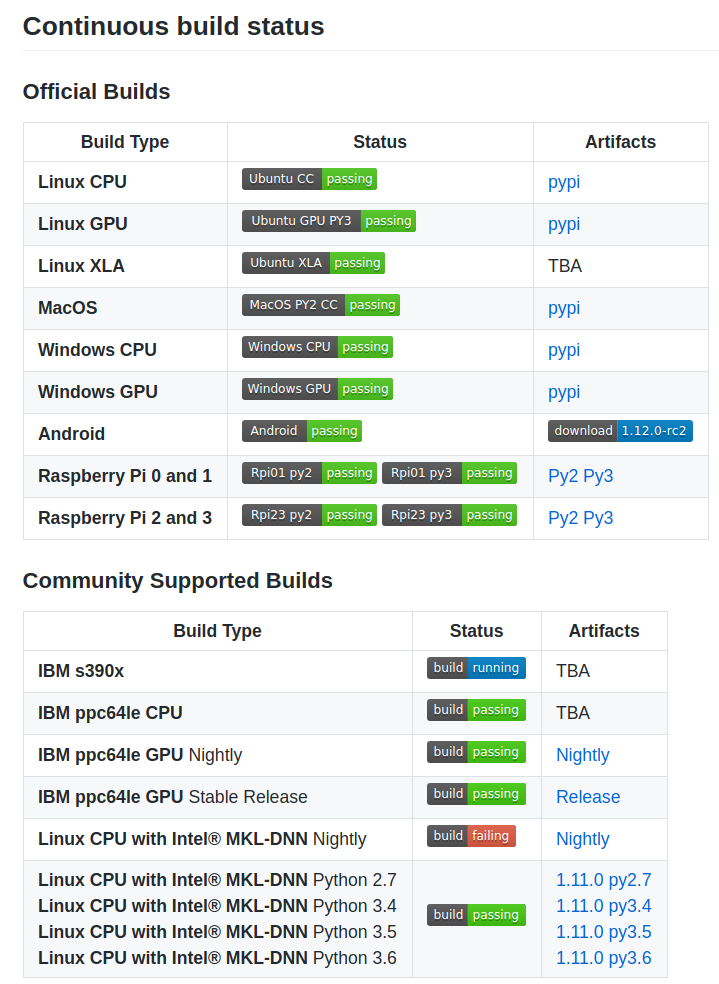
\includegraphics[width=0.7\linewidth]{content/chapter_testing/integration/continuousIntegration}
\end{center}
\end{Frame}
\subsection{System Testing}

\begin{Frame}{System Testing}
  \begin{itemize}
    \item Difficult, no (agreed) methodology.
    \item Divided into several categories:\newline
      \ \ -- Function testing, \newline
      \ \ -- volume and stress testing, \newline
      \ \ -- usability testing, \newline
      \ \ -- security testing, \newline
      \ \ -- performance testing, \newline
      \ \ -- installability testing and \newline
      \ \ -- recovery testing.
  \end{itemize}
\end{Frame}

\begin{Frame}{Function Testing}
  \begin{itemize}
    \item Does the system fulfill the functional specification?
    \item Create input data for the whole application and check \newline
      \ \ -- its output or\newline
      \ \ -- its behavior.
    \item Do not consider implementation details.
  \end{itemize}
\end{Frame}

\begin{Frame}{Volume and Stress Testing}
  \begin{itemize}
    \item Does the system work correctly in limit situations under \newline
      \ \ -- large volumes of data or\newline
      \ \ -- under high peak volumes of data?
    \item Limit situations: main memory or hard disk almost fully used.
  \end{itemize}
\end{Frame}

\begin{Frame}{Usability Testing}
  \begin{itemize}
    \item Are the error messages useful and understandable?
    \item Is the online-documentation adequate?
    \item Is the user interface adequate for different user types (novice, expert)?
    \item \ldots
  \end{itemize}
\end{Frame}

\begin{Frame}{Security Testing}
  \begin{itemize}
    \item Are access rights correctly implemented?
    \item Are transactions still correct under parallel access?
    \item \ldots
  \end{itemize}
\end{Frame}

\begin{Frame}{Performance Testing}
  \begin{itemize}
    \item Does the system meet the performance requirements?
    \item Possible requirements:\newline
      \ \ -- Transactions per second,\newline
      \ \ -- response time,\newline
      \ \ -- \ldots
  \end{itemize}
\end{Frame}
  
\begin{Frame}{Installability Testing}
  \begin{itemize}
    \item Can the system be installed in all
required environments?
    \item Are required dependencies available in all required environments?
    \item Is it compatible with other software?
    \item \ldots
  \end{itemize}
\end{Frame}

\begin{Frame}{Recovery Testing}
  \begin{itemize}
    \item Does the system recover well from a power cut?
    \item How much data is lost after the recovery?
    \item \ldots
  \end{itemize}
\end{Frame}


%!TEX root = ../../main.tex

\section{Conclusion}

\begin{frame}{Conclusion}
\begin{itemize}
\itemsep1em
\item Model Checking is an \hl{automatic} approach to \hl{verify} whether a given system satisfies a given specification
\item Proof of \hl{correctness} or \hl{counterexample} 
\item System properties: \hl{liveness, safety, invariants}
\item Symbolic Model Checking: make possible to handle infinite state systems and work around the state explosion problem
\item Over-/Under-approximation to abstract away superfluous information
\item Software Model Checking: no algorithm for all cases $\rightarrow$ combine different approaches    
\end{itemize}

\end{frame}
\subsection{Testing Summary}

\begin{Frame}{Testing Summary}{The Definition}
  \begin{definition}[Testing]
    \Def{Testing} is the examination of \alert{a subset} of the behaviors of a program or system.
  \end{definition}

  \xxx

  Testing can detect the presence of errors, but cannot prove their absence.
\end{Frame}



\begin{Frame}[fragile]{Testing in the V Model}
  \newcommand{\define}[1]{\inhead{#1} \\ \scriptsize define test cases}
  \newcommand{\code}{\inhead{Coding} \\ \scriptsize write code}
  \newcommand{\run}[1]{\inhead{#1} \\ \scriptsize run test cases}

  \begin{tikzpicture}[
    state/.style={
      draw=maincolor,
      thick,
      fill=maincolor!18,
      text width=2.5cm,
      align=center,
      font=\linespread{0.7}\selectfont,
      minimum height=8mm
    },
    heigh state/.style={
      state,
      minimum height=12mm
    },
    node distance=5mm and -2.2cm
  ]
    \node[heigh state] (define requirements) {\define{Requirements\\ Engineering}};
    \node[heigh state, below right=of define requirements] (define specification) {\define{Functional\\ Specification}};
    \node[state, below right=of define specification] (define system) {\define{System Design}};
    \node[state, below right=of define system] (define modules) {\define{Module Design}};
    \node[state, below right=5mm and -1cm of define modules] (code) {\code};
    \node[state, above right=5mm and -1cm of code] (test modules) {\run{Unit Test}};
    \node[state, above right=of test modules] (test system) {\run{Integration Test}};
    \node[heigh state, above right=of test system] (test specification) {\run{System Test}};
    \node[heigh state, above right=of test specification] (test requirements) {\run{Acceptance Test}};
    \path[very thick,maincolor,->]
      (define requirements) edge (define specification)
      (define specification) edge (define system)
      (define system) edge (define modules)
      (define modules) edge[shorten >=3pt] (code)
      (code) edge[shorten >=3pt] (test modules)
      (test modules) edge (test system)
      (test system) edge (test specification)
      (test specification) edge (test requirements);
    \path[dashed, thick,->,shorten <=3pt, shorten >=3pt,transform canvas={yshift=-2mm}]
      (define requirements) edge (test requirements)
      (define specification) edge (test specification)
      (define system) edge (test system)
      (define modules) edge (test modules);
  \end{tikzpicture}
\end{Frame}

\begin{Frame}{Levels of Automatization}
  \inhead{Code inspections} \\
    Manual testing based on knowledge and check lists. \hfill\vspace{1ex}\linebreak
  \inhead{Walkthroughs} \\
    Humans play computer. \hfill\vspace{1ex}\linebreak
  \inhead{Equivalence partitioning} \\
    Design test cases using equivalence classes.\hfill\vspace{1ex}\linebreak
  \inhead{Boundary values} \\
    Design test cases using boundaries of equivalence classes.\hfill\vspace{1ex}\linebreak
  \inhead{Path coverage} \\
    Design test cases by analyzing control-flow and data-flow.\hfill\vspace{1ex}\linebreak
  \inhead{Unit testing frameworks} \\
    Automatic test running, e.g. with JUnit\hfill\vspace{1ex}\linebreak
  \inhead{Weakest preconditions} \\
    (Semi-)Automatic test case design.
\end{Frame}








\mode<article>
\exercises

\mode
<all>